\documentclass[twoside]{book}

% Packages required by doxygen
\usepackage{fixltx2e}
\usepackage{calc}
\usepackage{doxygen}
\usepackage[export]{adjustbox} % also loads graphicx
\usepackage{graphicx}
\usepackage[utf8]{inputenc}
\usepackage{makeidx}
\usepackage{multicol}
\usepackage{multirow}
\PassOptionsToPackage{warn}{textcomp}
\usepackage{textcomp}
\usepackage[nointegrals]{wasysym}
\usepackage[table]{xcolor}

% Font selection
\usepackage[T1]{fontenc}
\usepackage[scaled=.90]{helvet}
\usepackage{courier}
\usepackage{amssymb}
\usepackage{sectsty}
\renewcommand{\familydefault}{\sfdefault}
\allsectionsfont{%
  \fontseries{bc}\selectfont%
  \color{darkgray}%
}
\renewcommand{\DoxyLabelFont}{%
  \fontseries{bc}\selectfont%
  \color{darkgray}%
}
\newcommand{\+}{\discretionary{\mbox{\scriptsize$\hookleftarrow$}}{}{}}

% Page & text layout
\usepackage{geometry}
\geometry{%
  a4paper,%
  top=2.5cm,%
  bottom=2.5cm,%
  left=2.5cm,%
  right=2.5cm%
}
\tolerance=750
\hfuzz=15pt
\hbadness=750
\setlength{\emergencystretch}{15pt}
\setlength{\parindent}{0cm}
\setlength{\parskip}{3ex plus 2ex minus 2ex}
\makeatletter
\renewcommand{\paragraph}{%
  \@startsection{paragraph}{4}{0ex}{-1.0ex}{1.0ex}{%
    \normalfont\normalsize\bfseries\SS@parafont%
  }%
}
\renewcommand{\subparagraph}{%
  \@startsection{subparagraph}{5}{0ex}{-1.0ex}{1.0ex}{%
    \normalfont\normalsize\bfseries\SS@subparafont%
  }%
}
\makeatother

% Headers & footers
\usepackage{fancyhdr}
\pagestyle{fancyplain}
\fancyhead[LE]{\fancyplain{}{\bfseries\thepage}}
\fancyhead[CE]{\fancyplain{}{}}
\fancyhead[RE]{\fancyplain{}{\bfseries\leftmark}}
\fancyhead[LO]{\fancyplain{}{\bfseries\rightmark}}
\fancyhead[CO]{\fancyplain{}{}}
\fancyhead[RO]{\fancyplain{}{\bfseries\thepage}}
\fancyfoot[LE]{\fancyplain{}{}}
\fancyfoot[CE]{\fancyplain{}{}}
\fancyfoot[RE]{\fancyplain{}{\bfseries\scriptsize Generated by Doxygen }}
\fancyfoot[LO]{\fancyplain{}{\bfseries\scriptsize Generated by Doxygen }}
\fancyfoot[CO]{\fancyplain{}{}}
\fancyfoot[RO]{\fancyplain{}{}}
\renewcommand{\footrulewidth}{0.4pt}
\renewcommand{\chaptermark}[1]{%
  \markboth{#1}{}%
}
\renewcommand{\sectionmark}[1]{%
  \markright{\thesection\ #1}%
}

% Indices & bibliography
\usepackage{natbib}
\usepackage[titles]{tocloft}
\setcounter{tocdepth}{3}
\setcounter{secnumdepth}{5}
\makeindex

% Hyperlinks (required, but should be loaded last)
\usepackage{ifpdf}
\ifpdf
  \usepackage[pdftex,pagebackref=true]{hyperref}
\else
  \usepackage[ps2pdf,pagebackref=true]{hyperref}
\fi
\hypersetup{%
  colorlinks=true,%
  linkcolor=blue,%
  citecolor=blue,%
  unicode%
}

% Custom commands
\newcommand{\clearemptydoublepage}{%
  \newpage{\pagestyle{empty}\cleardoublepage}%
}

\usepackage{caption}
\captionsetup{labelsep=space,justification=centering,font={bf},singlelinecheck=off,skip=4pt,position=top}

%===== C O N T E N T S =====

\begin{document}

% Titlepage & ToC
\hypersetup{pageanchor=false,
             bookmarksnumbered=true,
             pdfencoding=unicode
            }
\pagenumbering{alph}
\begin{titlepage}
\vspace*{7cm}
\begin{center}%
{\Large E\+N\+UM R\+O\+B\+OT \\[1ex]\large 1.\+0 }\\
\vspace*{1cm}
{\large Generated by Doxygen 1.8.13}\\
\end{center}
\end{titlepage}
\clearemptydoublepage
\pagenumbering{roman}
\tableofcontents
\clearemptydoublepage
\pagenumbering{arabic}
\hypersetup{pageanchor=true}

%--- Begin generated contents ---
\chapter{Example-\/\+Enum-\/\+Bot}
\label{md__r_e_a_d_m_e}
\Hypertarget{md__r_e_a_d_m_e}
\input{d3/dcc/md__r_e_a_d_m_e}
\chapter{Namespace Index}
\section{Packages}
Here are the packages with brief descriptions (if available)\+:\begin{DoxyCompactList}
\item\contentsline{section}{\hyperlink{namespacefrc}{frc} }{\pageref{namespacefrc}}{}
\item\contentsline{section}{\hyperlink{namespacefrc_1_1robot}{frc.\+robot} }{\pageref{namespacefrc_1_1robot}}{}
\item\contentsline{section}{\hyperlink{namespacefrc_1_1robot_1_1_enums}{frc.\+robot.\+Enums} }{\pageref{namespacefrc_1_1robot_1_1_enums}}{}
\item\contentsline{section}{\hyperlink{namespacefrc_1_1robot_1_1subsystems}{frc.\+robot.\+subsystems} }{\pageref{namespacefrc_1_1robot_1_1subsystems}}{}
\end{DoxyCompactList}

\chapter{Hierarchical Index}
\section{Class Hierarchy}
This inheritance list is sorted roughly, but not completely, alphabetically\+:\begin{DoxyCompactList}
\item \contentsline{section}{frc.\+robot.\+subsystems.\+Cargo}{\pageref{classfrc_1_1robot_1_1subsystems_1_1_cargo}}{}
\item \contentsline{section}{frc.\+robot.\+subsystems.\+Drive\+Train}{\pageref{classfrc_1_1robot_1_1subsystems_1_1_drive_train}}{}
\item \contentsline{section}{frc.\+robot.\+Enums.\+Hatch}{\pageref{enumfrc_1_1robot_1_1_enums_1_1_hatch}}{}
\item \contentsline{section}{frc.\+robot.\+subsystems.\+Hatch\+\_\+\+Control}{\pageref{classfrc_1_1robot_1_1subsystems_1_1_hatch___control}}{}
\item \contentsline{section}{frc.\+robot.\+Enums.\+Lift\+\_\+\+Pistons}{\pageref{enumfrc_1_1robot_1_1_enums_1_1_lift___pistons}}{}
\item \contentsline{section}{frc.\+robot.\+Main}{\pageref{classfrc_1_1robot_1_1_main}}{}
\item \contentsline{section}{frc.\+robot.\+OI}{\pageref{classfrc_1_1robot_1_1_o_i}}{}
\item \contentsline{section}{frc.\+robot.\+Robot\+Map}{\pageref{classfrc_1_1robot_1_1_robot_map}}{}
\item \contentsline{section}{frc.\+robot.\+Enums.\+Shift}{\pageref{enumfrc_1_1robot_1_1_enums_1_1_shift}}{}
\item \contentsline{section}{frc.\+robot.\+subsystems.\+Stilts}{\pageref{classfrc_1_1robot_1_1subsystems_1_1_stilts}}{}
\item \contentsline{section}{frc.\+robot.\+subsystems.\+Teleop}{\pageref{classfrc_1_1robot_1_1subsystems_1_1_teleop}}{}
\item \contentsline{section}{frc.\+robot.\+subsystems.\+Teleop\+\_\+\+Controller2}{\pageref{classfrc_1_1robot_1_1subsystems_1_1_teleop___controller2}}{}
\item Timed\+Robot\begin{DoxyCompactList}
\item \contentsline{section}{frc.\+robot.\+Robot}{\pageref{classfrc_1_1robot_1_1_robot}}{}
\end{DoxyCompactList}
\end{DoxyCompactList}

\chapter{Class Index}
\section{Class List}
Here are the classes, structs, unions and interfaces with brief descriptions\+:\begin{DoxyCompactList}
\item\contentsline{section}{\hyperlink{classfrc_1_1robot_1_1subsystems_1_1_cargo}{frc.\+robot.\+subsystems.\+Cargo} }{\pageref{classfrc_1_1robot_1_1subsystems_1_1_cargo}}{}
\item\contentsline{section}{\hyperlink{classfrc_1_1robot_1_1subsystems_1_1_drive_train}{frc.\+robot.\+subsystems.\+Drive\+Train} }{\pageref{classfrc_1_1robot_1_1subsystems_1_1_drive_train}}{}
\item\contentsline{section}{\hyperlink{enumfrc_1_1robot_1_1_enums_1_1_hatch}{frc.\+robot.\+Enums.\+Hatch} }{\pageref{enumfrc_1_1robot_1_1_enums_1_1_hatch}}{}
\item\contentsline{section}{\hyperlink{classfrc_1_1robot_1_1subsystems_1_1_hatch___control}{frc.\+robot.\+subsystems.\+Hatch\+\_\+\+Control} }{\pageref{classfrc_1_1robot_1_1subsystems_1_1_hatch___control}}{}
\item\contentsline{section}{\hyperlink{enumfrc_1_1robot_1_1_enums_1_1_lift___pistons}{frc.\+robot.\+Enums.\+Lift\+\_\+\+Pistons} }{\pageref{enumfrc_1_1robot_1_1_enums_1_1_lift___pistons}}{}
\item\contentsline{section}{\hyperlink{classfrc_1_1robot_1_1_main}{frc.\+robot.\+Main} \\*Do N\+OT add any static variables to this class, or any initialization at all }{\pageref{classfrc_1_1robot_1_1_main}}{}
\item\contentsline{section}{\hyperlink{classfrc_1_1robot_1_1_o_i}{frc.\+robot.\+OI} \\*This class is the glue that binds the controls on the physical operator interface to the commands and command groups that allow control of the robot }{\pageref{classfrc_1_1robot_1_1_o_i}}{}
\item\contentsline{section}{\hyperlink{classfrc_1_1robot_1_1_robot}{frc.\+robot.\+Robot} }{\pageref{classfrc_1_1robot_1_1_robot}}{}
\item\contentsline{section}{\hyperlink{classfrc_1_1robot_1_1_robot_map}{frc.\+robot.\+Robot\+Map} \\*The \hyperlink{classfrc_1_1robot_1_1_robot_map}{Robot\+Map} is a mapping from the ports sensors and actuators are wired into to a variable name }{\pageref{classfrc_1_1robot_1_1_robot_map}}{}
\item\contentsline{section}{\hyperlink{enumfrc_1_1robot_1_1_enums_1_1_shift}{frc.\+robot.\+Enums.\+Shift} }{\pageref{enumfrc_1_1robot_1_1_enums_1_1_shift}}{}
\item\contentsline{section}{\hyperlink{classfrc_1_1robot_1_1subsystems_1_1_stilts}{frc.\+robot.\+subsystems.\+Stilts} }{\pageref{classfrc_1_1robot_1_1subsystems_1_1_stilts}}{}
\item\contentsline{section}{\hyperlink{classfrc_1_1robot_1_1subsystems_1_1_teleop}{frc.\+robot.\+subsystems.\+Teleop} }{\pageref{classfrc_1_1robot_1_1subsystems_1_1_teleop}}{}
\item\contentsline{section}{\hyperlink{classfrc_1_1robot_1_1subsystems_1_1_teleop___controller2}{frc.\+robot.\+subsystems.\+Teleop\+\_\+\+Controller2} }{\pageref{classfrc_1_1robot_1_1subsystems_1_1_teleop___controller2}}{}
\end{DoxyCompactList}

\chapter{File Index}
\section{File List}
Here is a list of all files with brief descriptions\+:\begin{DoxyCompactList}
\item\contentsline{section}{src/main/java/frc/robot/\hyperlink{_main_8java}{Main.\+java} }{\pageref{_main_8java}}{}
\item\contentsline{section}{src/main/java/frc/robot/\hyperlink{_o_i_8java}{O\+I.\+java} }{\pageref{_o_i_8java}}{}
\item\contentsline{section}{src/main/java/frc/robot/\hyperlink{_robot_8java}{Robot.\+java} }{\pageref{_robot_8java}}{}
\item\contentsline{section}{src/main/java/frc/robot/\hyperlink{_robot_map_8java}{Robot\+Map.\+java} }{\pageref{_robot_map_8java}}{}
\item\contentsline{section}{src/main/java/frc/robot/\+Enums/\hyperlink{_hatch_8java}{Hatch.\+java} }{\pageref{_hatch_8java}}{}
\item\contentsline{section}{src/main/java/frc/robot/\+Enums/\hyperlink{_lift___pistons_8java}{Lift\+\_\+\+Pistons.\+java} }{\pageref{_lift___pistons_8java}}{}
\item\contentsline{section}{src/main/java/frc/robot/\+Enums/\hyperlink{_shift_8java}{Shift.\+java} }{\pageref{_shift_8java}}{}
\item\contentsline{section}{src/main/java/frc/robot/subsystems/\hyperlink{_cargo_8java}{Cargo.\+java} }{\pageref{_cargo_8java}}{}
\item\contentsline{section}{src/main/java/frc/robot/subsystems/\hyperlink{_drive_train_8java}{Drive\+Train.\+java} }{\pageref{_drive_train_8java}}{}
\item\contentsline{section}{src/main/java/frc/robot/subsystems/\hyperlink{_hatch___control_8java}{Hatch\+\_\+\+Control.\+java} }{\pageref{_hatch___control_8java}}{}
\item\contentsline{section}{src/main/java/frc/robot/subsystems/\hyperlink{_stilts_8java}{Stilts.\+java} }{\pageref{_stilts_8java}}{}
\item\contentsline{section}{src/main/java/frc/robot/subsystems/\hyperlink{_teleop_8java}{Teleop.\+java} }{\pageref{_teleop_8java}}{}
\item\contentsline{section}{src/main/java/frc/robot/subsystems/\hyperlink{_teleop___controller2_8java}{Teleop\+\_\+\+Controller2.\+java} }{\pageref{_teleop___controller2_8java}}{}
\end{DoxyCompactList}

\chapter{Namespace Documentation}
\hypertarget{namespacefrc}{}\section{Package frc}
\label{namespacefrc}\index{frc@{frc}}
\subsection*{Packages}
\begin{DoxyCompactItemize}
\item 
package \hyperlink{namespacefrc_1_1robot}{robot}
\end{DoxyCompactItemize}

\hypertarget{namespacefrc_1_1robot}{}\section{Package frc.\+robot}
\label{namespacefrc_1_1robot}\index{frc.\+robot@{frc.\+robot}}
\subsection*{Packages}
\begin{DoxyCompactItemize}
\item 
package \hyperlink{namespacefrc_1_1robot_1_1Enums}{Enums}
\item 
package \hyperlink{namespacefrc_1_1robot_1_1subsystems}{subsystems}
\end{DoxyCompactItemize}
\subsection*{Classes}
\begin{DoxyCompactItemize}
\item 
class \hyperlink{classfrc_1_1robot_1_1Main}{Main}
\begin{DoxyCompactList}\small\item\em Do N\+OT add any static variables to this class, or any initialization at all. \end{DoxyCompactList}\item 
class \hyperlink{classfrc_1_1robot_1_1OI}{OI}
\begin{DoxyCompactList}\small\item\em This class is the glue that binds the controls on the physical operator interface to the commands and command groups that allow control of the robot. \end{DoxyCompactList}\item 
class \hyperlink{classfrc_1_1robot_1_1Robot}{Robot}
\item 
class \hyperlink{classfrc_1_1robot_1_1RobotMap}{Robot\+Map}
\begin{DoxyCompactList}\small\item\em The \hyperlink{classfrc_1_1robot_1_1RobotMap}{Robot\+Map} is a mapping from the ports sensors and actuators are wired into to a variable name. \end{DoxyCompactList}\end{DoxyCompactItemize}

\hypertarget{namespacefrc_1_1robot_1_1_enums}{}\section{Package frc.\+robot.\+Enums}
\label{namespacefrc_1_1robot_1_1_enums}\index{frc.\+robot.\+Enums@{frc.\+robot.\+Enums}}
\subsection*{Classes}
\begin{DoxyCompactItemize}
\item 
enum \hyperlink{enumfrc_1_1robot_1_1_enums_1_1_hatch}{Hatch}
\item 
enum \hyperlink{enumfrc_1_1robot_1_1_enums_1_1_lift___pistons}{Lift\+\_\+\+Pistons}
\item 
enum \hyperlink{enumfrc_1_1robot_1_1_enums_1_1_shift}{Shift}
\end{DoxyCompactItemize}

\hypertarget{namespacefrc_1_1robot_1_1subsystems}{}\section{Package frc.\+robot.\+subsystems}
\label{namespacefrc_1_1robot_1_1subsystems}\index{frc.\+robot.\+subsystems@{frc.\+robot.\+subsystems}}
\subsection*{Classes}
\begin{DoxyCompactItemize}
\item 
class \hyperlink{classfrc_1_1robot_1_1subsystems_1_1Cargo}{Cargo}
\item 
class \hyperlink{classfrc_1_1robot_1_1subsystems_1_1DriveTrain}{Drive\+Train}
\item 
class \hyperlink{classfrc_1_1robot_1_1subsystems_1_1Hatch__Control}{Hatch\+\_\+\+Control}
\item 
class \hyperlink{classfrc_1_1robot_1_1subsystems_1_1Stilts}{Stilts}
\item 
class \hyperlink{classfrc_1_1robot_1_1subsystems_1_1Teleop}{Teleop}
\item 
class \hyperlink{classfrc_1_1robot_1_1subsystems_1_1Teleop__Controller2}{Teleop\+\_\+\+Controller2}
\end{DoxyCompactItemize}

\chapter{Class Documentation}
\hypertarget{classfrc_1_1robot_1_1subsystems_1_1_cargo}{}\section{frc.\+robot.\+subsystems.\+Cargo Class Reference}
\label{classfrc_1_1robot_1_1subsystems_1_1_cargo}\index{frc.\+robot.\+subsystems.\+Cargo@{frc.\+robot.\+subsystems.\+Cargo}}


Collaboration diagram for frc.\+robot.\+subsystems.\+Cargo\+:\nopagebreak
\begin{figure}[H]
\begin{center}
\leavevmode
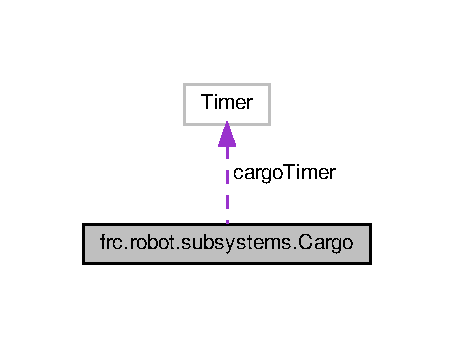
\includegraphics[width=218pt]{de/d2d/classfrc_1_1robot_1_1subsystems_1_1_cargo__coll__graph}
\end{center}
\end{figure}
\subsection*{Public Member Functions}
\begin{DoxyCompactItemize}
\item 
\hyperlink{classfrc_1_1robot_1_1subsystems_1_1_cargo_ad27213bb1c8c9a33d5c2b9cc153c1508}{Cargo} ()
\end{DoxyCompactItemize}
\subsection*{Static Public Member Functions}
\begin{DoxyCompactItemize}
\item 
static void \hyperlink{classfrc_1_1robot_1_1subsystems_1_1_cargo_aa8640bc75e8b3f2472ea586936d6ed1f}{actuate\+Arm} (double speed)
\item 
static void \hyperlink{classfrc_1_1robot_1_1subsystems_1_1_cargo_aa85a0b3aa7cb498f4b1c7eac6d26bce2}{stop\+Arm} ()
\item 
static void \hyperlink{classfrc_1_1robot_1_1subsystems_1_1_cargo_aa05df516e815067a7b853d9fbdc35f01}{actuate\+Claw} (double speed)
\item 
static void \hyperlink{classfrc_1_1robot_1_1subsystems_1_1_cargo_a0ac97ff2fa2f7af96744a5dcba7ba61b}{stop\+Claw} ()
\item 
static void \hyperlink{classfrc_1_1robot_1_1subsystems_1_1_cargo_a8a4dd09c62967c4d82af8953cf8ab731}{hold\+Ball} ()
\item 
static void \hyperlink{classfrc_1_1robot_1_1subsystems_1_1_cargo_a20e8230acdc07d7d94e056f9e09d91ad}{update} ()
\end{DoxyCompactItemize}
\subsection*{Static Public Attributes}
\begin{DoxyCompactItemize}
\item 
static Timer \hyperlink{classfrc_1_1robot_1_1subsystems_1_1_cargo_a50722902fa0c3ad0db5f592ad51b94f6}{cargo\+Timer} = new Timer()
\end{DoxyCompactItemize}


\subsection{Detailed Description}


Definition at line 7 of file Cargo.\+java.



\subsection{Constructor \& Destructor Documentation}
\mbox{\Hypertarget{classfrc_1_1robot_1_1subsystems_1_1_cargo_ad27213bb1c8c9a33d5c2b9cc153c1508}\label{classfrc_1_1robot_1_1subsystems_1_1_cargo_ad27213bb1c8c9a33d5c2b9cc153c1508}} 
\index{frc\+::robot\+::subsystems\+::\+Cargo@{frc\+::robot\+::subsystems\+::\+Cargo}!Cargo@{Cargo}}
\index{Cargo@{Cargo}!frc\+::robot\+::subsystems\+::\+Cargo@{frc\+::robot\+::subsystems\+::\+Cargo}}
\subsubsection{\texorpdfstring{Cargo()}{Cargo()}}
{\footnotesize\ttfamily frc.\+robot.\+subsystems.\+Cargo.\+Cargo (\begin{DoxyParamCaption}{ }\end{DoxyParamCaption})}



Definition at line 13 of file Cargo.\+java.



\subsection{Member Function Documentation}
\mbox{\Hypertarget{classfrc_1_1robot_1_1subsystems_1_1_cargo_aa8640bc75e8b3f2472ea586936d6ed1f}\label{classfrc_1_1robot_1_1subsystems_1_1_cargo_aa8640bc75e8b3f2472ea586936d6ed1f}} 
\index{frc\+::robot\+::subsystems\+::\+Cargo@{frc\+::robot\+::subsystems\+::\+Cargo}!actuate\+Arm@{actuate\+Arm}}
\index{actuate\+Arm@{actuate\+Arm}!frc\+::robot\+::subsystems\+::\+Cargo@{frc\+::robot\+::subsystems\+::\+Cargo}}
\subsubsection{\texorpdfstring{actuate\+Arm()}{actuateArm()}}
{\footnotesize\ttfamily static void frc.\+robot.\+subsystems.\+Cargo.\+actuate\+Arm (\begin{DoxyParamCaption}\item[{double}]{speed }\end{DoxyParamCaption})\hspace{0.3cm}{\ttfamily [static]}}



Definition at line 14 of file Cargo.\+java.

\mbox{\Hypertarget{classfrc_1_1robot_1_1subsystems_1_1_cargo_aa05df516e815067a7b853d9fbdc35f01}\label{classfrc_1_1robot_1_1subsystems_1_1_cargo_aa05df516e815067a7b853d9fbdc35f01}} 
\index{frc\+::robot\+::subsystems\+::\+Cargo@{frc\+::robot\+::subsystems\+::\+Cargo}!actuate\+Claw@{actuate\+Claw}}
\index{actuate\+Claw@{actuate\+Claw}!frc\+::robot\+::subsystems\+::\+Cargo@{frc\+::robot\+::subsystems\+::\+Cargo}}
\subsubsection{\texorpdfstring{actuate\+Claw()}{actuateClaw()}}
{\footnotesize\ttfamily static void frc.\+robot.\+subsystems.\+Cargo.\+actuate\+Claw (\begin{DoxyParamCaption}\item[{double}]{speed }\end{DoxyParamCaption})\hspace{0.3cm}{\ttfamily [static]}}



Definition at line 20 of file Cargo.\+java.

\mbox{\Hypertarget{classfrc_1_1robot_1_1subsystems_1_1_cargo_a8a4dd09c62967c4d82af8953cf8ab731}\label{classfrc_1_1robot_1_1subsystems_1_1_cargo_a8a4dd09c62967c4d82af8953cf8ab731}} 
\index{frc\+::robot\+::subsystems\+::\+Cargo@{frc\+::robot\+::subsystems\+::\+Cargo}!hold\+Ball@{hold\+Ball}}
\index{hold\+Ball@{hold\+Ball}!frc\+::robot\+::subsystems\+::\+Cargo@{frc\+::robot\+::subsystems\+::\+Cargo}}
\subsubsection{\texorpdfstring{hold\+Ball()}{holdBall()}}
{\footnotesize\ttfamily static void frc.\+robot.\+subsystems.\+Cargo.\+hold\+Ball (\begin{DoxyParamCaption}{ }\end{DoxyParamCaption})\hspace{0.3cm}{\ttfamily [static]}}



Definition at line 26 of file Cargo.\+java.

\mbox{\Hypertarget{classfrc_1_1robot_1_1subsystems_1_1_cargo_aa85a0b3aa7cb498f4b1c7eac6d26bce2}\label{classfrc_1_1robot_1_1subsystems_1_1_cargo_aa85a0b3aa7cb498f4b1c7eac6d26bce2}} 
\index{frc\+::robot\+::subsystems\+::\+Cargo@{frc\+::robot\+::subsystems\+::\+Cargo}!stop\+Arm@{stop\+Arm}}
\index{stop\+Arm@{stop\+Arm}!frc\+::robot\+::subsystems\+::\+Cargo@{frc\+::robot\+::subsystems\+::\+Cargo}}
\subsubsection{\texorpdfstring{stop\+Arm()}{stopArm()}}
{\footnotesize\ttfamily static void frc.\+robot.\+subsystems.\+Cargo.\+stop\+Arm (\begin{DoxyParamCaption}{ }\end{DoxyParamCaption})\hspace{0.3cm}{\ttfamily [static]}}



Definition at line 17 of file Cargo.\+java.

\mbox{\Hypertarget{classfrc_1_1robot_1_1subsystems_1_1_cargo_a0ac97ff2fa2f7af96744a5dcba7ba61b}\label{classfrc_1_1robot_1_1subsystems_1_1_cargo_a0ac97ff2fa2f7af96744a5dcba7ba61b}} 
\index{frc\+::robot\+::subsystems\+::\+Cargo@{frc\+::robot\+::subsystems\+::\+Cargo}!stop\+Claw@{stop\+Claw}}
\index{stop\+Claw@{stop\+Claw}!frc\+::robot\+::subsystems\+::\+Cargo@{frc\+::robot\+::subsystems\+::\+Cargo}}
\subsubsection{\texorpdfstring{stop\+Claw()}{stopClaw()}}
{\footnotesize\ttfamily static void frc.\+robot.\+subsystems.\+Cargo.\+stop\+Claw (\begin{DoxyParamCaption}{ }\end{DoxyParamCaption})\hspace{0.3cm}{\ttfamily [static]}}



Definition at line 23 of file Cargo.\+java.

\mbox{\Hypertarget{classfrc_1_1robot_1_1subsystems_1_1_cargo_a20e8230acdc07d7d94e056f9e09d91ad}\label{classfrc_1_1robot_1_1subsystems_1_1_cargo_a20e8230acdc07d7d94e056f9e09d91ad}} 
\index{frc\+::robot\+::subsystems\+::\+Cargo@{frc\+::robot\+::subsystems\+::\+Cargo}!update@{update}}
\index{update@{update}!frc\+::robot\+::subsystems\+::\+Cargo@{frc\+::robot\+::subsystems\+::\+Cargo}}
\subsubsection{\texorpdfstring{update()}{update()}}
{\footnotesize\ttfamily static void frc.\+robot.\+subsystems.\+Cargo.\+update (\begin{DoxyParamCaption}{ }\end{DoxyParamCaption})\hspace{0.3cm}{\ttfamily [static]}}



Definition at line 29 of file Cargo.\+java.

Here is the call graph for this function\+:\nopagebreak
\begin{figure}[H]
\begin{center}
\leavevmode
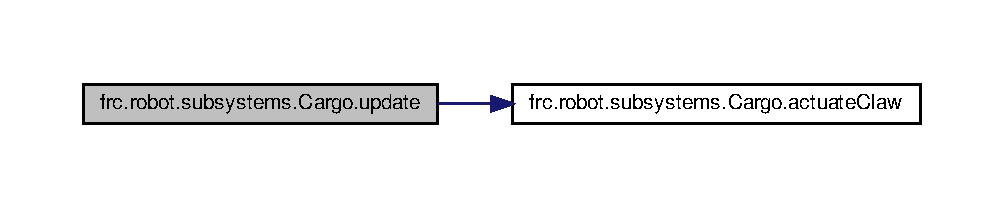
\includegraphics[width=350pt]{d6/dae/classfrc_1_1robot_1_1subsystems_1_1_cargo_a20e8230acdc07d7d94e056f9e09d91ad_cgraph}
\end{center}
\end{figure}


\subsection{Member Data Documentation}
\mbox{\Hypertarget{classfrc_1_1robot_1_1subsystems_1_1_cargo_a50722902fa0c3ad0db5f592ad51b94f6}\label{classfrc_1_1robot_1_1subsystems_1_1_cargo_a50722902fa0c3ad0db5f592ad51b94f6}} 
\index{frc\+::robot\+::subsystems\+::\+Cargo@{frc\+::robot\+::subsystems\+::\+Cargo}!cargo\+Timer@{cargo\+Timer}}
\index{cargo\+Timer@{cargo\+Timer}!frc\+::robot\+::subsystems\+::\+Cargo@{frc\+::robot\+::subsystems\+::\+Cargo}}
\subsubsection{\texorpdfstring{cargo\+Timer}{cargoTimer}}
{\footnotesize\ttfamily Timer frc.\+robot.\+subsystems.\+Cargo.\+cargo\+Timer = new Timer()\hspace{0.3cm}{\ttfamily [static]}}



Definition at line 8 of file Cargo.\+java.



The documentation for this class was generated from the following file\+:\begin{DoxyCompactItemize}
\item 
src/main/java/frc/robot/subsystems/\hyperlink{_cargo_8java}{Cargo.\+java}\end{DoxyCompactItemize}

\hypertarget{classfrc_1_1robot_1_1subsystems_1_1_drive_train}{}\section{frc.\+robot.\+subsystems.\+Drive\+Train Class Reference}
\label{classfrc_1_1robot_1_1subsystems_1_1_drive_train}\index{frc.\+robot.\+subsystems.\+Drive\+Train@{frc.\+robot.\+subsystems.\+Drive\+Train}}
\subsection*{Static Public Member Functions}
\begin{DoxyCompactItemize}
\item 
\mbox{\Hypertarget{classfrc_1_1robot_1_1subsystems_1_1_drive_train_a3288b5af8182d08f76290b257041538c}\label{classfrc_1_1robot_1_1subsystems_1_1_drive_train_a3288b5af8182d08f76290b257041538c}} 
static void {\bfseries shift} (\hyperlink{enumfrc_1_1robot_1_1_enums_1_1_shift}{Shift} direction)
\item 
\mbox{\Hypertarget{classfrc_1_1robot_1_1subsystems_1_1_drive_train_a883baac3715e22887c0ec5ce825fbfab}\label{classfrc_1_1robot_1_1subsystems_1_1_drive_train_a883baac3715e22887c0ec5ce825fbfab}} 
static void {\bfseries periodic} ()
\end{DoxyCompactItemize}


The documentation for this class was generated from the following file\+:\begin{DoxyCompactItemize}
\item 
src/main/java/frc/robot/subsystems/Drive\+Train.\+java\end{DoxyCompactItemize}

\hypertarget{enumfrc_1_1robot_1_1_enums_1_1_hatch}{}\section{frc.\+robot.\+Enums.\+Hatch Enum Reference}
\label{enumfrc_1_1robot_1_1_enums_1_1_hatch}\index{frc.\+robot.\+Enums.\+Hatch@{frc.\+robot.\+Enums.\+Hatch}}
\subsection*{Public Attributes}
\begin{DoxyCompactItemize}
\item 
\hyperlink{enumfrc_1_1robot_1_1_enums_1_1_hatch_aa9182f52be77e783bb38e7cfbf5bb700}{Extend}
\item 
\hyperlink{enumfrc_1_1robot_1_1_enums_1_1_hatch_ac4881a7e4ca2bc7c64aa8acd0da91d6e}{Retract}
\item 
\hyperlink{enumfrc_1_1robot_1_1_enums_1_1_hatch_aba378e125bbd0e4206aa27ab9bc51b0b}{Open}
\item 
\hyperlink{enumfrc_1_1robot_1_1_enums_1_1_hatch_ad9de6151d633f63ba3cb50aaeba1afd0}{Close}
\end{DoxyCompactItemize}


\subsection{Detailed Description}


Definition at line 4 of file Hatch.\+java.



\subsection{Member Data Documentation}
\mbox{\Hypertarget{enumfrc_1_1robot_1_1_enums_1_1_hatch_ad9de6151d633f63ba3cb50aaeba1afd0}\label{enumfrc_1_1robot_1_1_enums_1_1_hatch_ad9de6151d633f63ba3cb50aaeba1afd0}} 
\index{frc\+::robot\+::\+Enums\+::\+Hatch@{frc\+::robot\+::\+Enums\+::\+Hatch}!Close@{Close}}
\index{Close@{Close}!frc\+::robot\+::\+Enums\+::\+Hatch@{frc\+::robot\+::\+Enums\+::\+Hatch}}
\subsubsection{\texorpdfstring{Close}{Close}}
{\footnotesize\ttfamily frc.\+robot.\+Enums.\+Hatch.\+Close}



Definition at line 8 of file Hatch.\+java.

\mbox{\Hypertarget{enumfrc_1_1robot_1_1_enums_1_1_hatch_aa9182f52be77e783bb38e7cfbf5bb700}\label{enumfrc_1_1robot_1_1_enums_1_1_hatch_aa9182f52be77e783bb38e7cfbf5bb700}} 
\index{frc\+::robot\+::\+Enums\+::\+Hatch@{frc\+::robot\+::\+Enums\+::\+Hatch}!Extend@{Extend}}
\index{Extend@{Extend}!frc\+::robot\+::\+Enums\+::\+Hatch@{frc\+::robot\+::\+Enums\+::\+Hatch}}
\subsubsection{\texorpdfstring{Extend}{Extend}}
{\footnotesize\ttfamily frc.\+robot.\+Enums.\+Hatch.\+Extend}



Definition at line 5 of file Hatch.\+java.

\mbox{\Hypertarget{enumfrc_1_1robot_1_1_enums_1_1_hatch_aba378e125bbd0e4206aa27ab9bc51b0b}\label{enumfrc_1_1robot_1_1_enums_1_1_hatch_aba378e125bbd0e4206aa27ab9bc51b0b}} 
\index{frc\+::robot\+::\+Enums\+::\+Hatch@{frc\+::robot\+::\+Enums\+::\+Hatch}!Open@{Open}}
\index{Open@{Open}!frc\+::robot\+::\+Enums\+::\+Hatch@{frc\+::robot\+::\+Enums\+::\+Hatch}}
\subsubsection{\texorpdfstring{Open}{Open}}
{\footnotesize\ttfamily frc.\+robot.\+Enums.\+Hatch.\+Open}



Definition at line 7 of file Hatch.\+java.

\mbox{\Hypertarget{enumfrc_1_1robot_1_1_enums_1_1_hatch_ac4881a7e4ca2bc7c64aa8acd0da91d6e}\label{enumfrc_1_1robot_1_1_enums_1_1_hatch_ac4881a7e4ca2bc7c64aa8acd0da91d6e}} 
\index{frc\+::robot\+::\+Enums\+::\+Hatch@{frc\+::robot\+::\+Enums\+::\+Hatch}!Retract@{Retract}}
\index{Retract@{Retract}!frc\+::robot\+::\+Enums\+::\+Hatch@{frc\+::robot\+::\+Enums\+::\+Hatch}}
\subsubsection{\texorpdfstring{Retract}{Retract}}
{\footnotesize\ttfamily frc.\+robot.\+Enums.\+Hatch.\+Retract}



Definition at line 6 of file Hatch.\+java.



The documentation for this enum was generated from the following file\+:\begin{DoxyCompactItemize}
\item 
src/main/java/frc/robot/\+Enums/\hyperlink{_hatch_8java}{Hatch.\+java}\end{DoxyCompactItemize}

\hypertarget{classfrc_1_1robot_1_1subsystems_1_1_hatch___control}{}\section{frc.\+robot.\+subsystems.\+Hatch\+\_\+\+Control Class Reference}
\label{classfrc_1_1robot_1_1subsystems_1_1_hatch___control}\index{frc.\+robot.\+subsystems.\+Hatch\+\_\+\+Control@{frc.\+robot.\+subsystems.\+Hatch\+\_\+\+Control}}
\subsection*{Static Public Member Functions}
\begin{DoxyCompactItemize}
\item 
static void \hyperlink{classfrc_1_1robot_1_1subsystems_1_1_hatch___control_a10439efd71fc486d24b95364d70dcde3}{Tilt} (\hyperlink{enumfrc_1_1robot_1_1_enums_1_1_hatch}{Hatch} hatch)
\item 
static void \hyperlink{classfrc_1_1robot_1_1subsystems_1_1_hatch___control_a902c47bda22ebf4421953aafbc76128e}{mainip} (\hyperlink{enumfrc_1_1robot_1_1_enums_1_1_hatch}{Hatch} Manip)
\end{DoxyCompactItemize}


\subsection{Detailed Description}


Definition at line 11 of file Hatch\+\_\+\+Control.\+java.



\subsection{Member Function Documentation}
\mbox{\Hypertarget{classfrc_1_1robot_1_1subsystems_1_1_hatch___control_a902c47bda22ebf4421953aafbc76128e}\label{classfrc_1_1robot_1_1subsystems_1_1_hatch___control_a902c47bda22ebf4421953aafbc76128e}} 
\index{frc\+::robot\+::subsystems\+::\+Hatch\+\_\+\+Control@{frc\+::robot\+::subsystems\+::\+Hatch\+\_\+\+Control}!mainip@{mainip}}
\index{mainip@{mainip}!frc\+::robot\+::subsystems\+::\+Hatch\+\_\+\+Control@{frc\+::robot\+::subsystems\+::\+Hatch\+\_\+\+Control}}
\subsubsection{\texorpdfstring{mainip()}{mainip()}}
{\footnotesize\ttfamily static void frc.\+robot.\+subsystems.\+Hatch\+\_\+\+Control.\+mainip (\begin{DoxyParamCaption}\item[{\hyperlink{enumfrc_1_1robot_1_1_enums_1_1_hatch}{Hatch}}]{Manip }\end{DoxyParamCaption})\hspace{0.3cm}{\ttfamily [static]}}



Definition at line 30 of file Hatch\+\_\+\+Control.\+java.

\mbox{\Hypertarget{classfrc_1_1robot_1_1subsystems_1_1_hatch___control_a10439efd71fc486d24b95364d70dcde3}\label{classfrc_1_1robot_1_1subsystems_1_1_hatch___control_a10439efd71fc486d24b95364d70dcde3}} 
\index{frc\+::robot\+::subsystems\+::\+Hatch\+\_\+\+Control@{frc\+::robot\+::subsystems\+::\+Hatch\+\_\+\+Control}!Tilt@{Tilt}}
\index{Tilt@{Tilt}!frc\+::robot\+::subsystems\+::\+Hatch\+\_\+\+Control@{frc\+::robot\+::subsystems\+::\+Hatch\+\_\+\+Control}}
\subsubsection{\texorpdfstring{Tilt()}{Tilt()}}
{\footnotesize\ttfamily static void frc.\+robot.\+subsystems.\+Hatch\+\_\+\+Control.\+Tilt (\begin{DoxyParamCaption}\item[{\hyperlink{enumfrc_1_1robot_1_1_enums_1_1_hatch}{Hatch}}]{hatch }\end{DoxyParamCaption})\hspace{0.3cm}{\ttfamily [static]}}



Definition at line 12 of file Hatch\+\_\+\+Control.\+java.



The documentation for this class was generated from the following file\+:\begin{DoxyCompactItemize}
\item 
src/main/java/frc/robot/subsystems/\hyperlink{_hatch___control_8java}{Hatch\+\_\+\+Control.\+java}\end{DoxyCompactItemize}

\hypertarget{enumfrc_1_1robot_1_1_enums_1_1_lift___pistons}{}\section{frc.\+robot.\+Enums.\+Lift\+\_\+\+Pistons Enum Reference}
\label{enumfrc_1_1robot_1_1_enums_1_1_lift___pistons}\index{frc.\+robot.\+Enums.\+Lift\+\_\+\+Pistons@{frc.\+robot.\+Enums.\+Lift\+\_\+\+Pistons}}
\subsection*{Public Attributes}
\begin{DoxyCompactItemize}
\item 
\hyperlink{enumfrc_1_1robot_1_1_enums_1_1_lift___pistons_a6330e41bb1e82289bb679d21e466cb04}{Extend}
\item 
\hyperlink{enumfrc_1_1robot_1_1_enums_1_1_lift___pistons_a95ac3a721cf39027b6e0bd0ea87f2a13}{Retract}
\end{DoxyCompactItemize}


\subsection{Detailed Description}


Definition at line 3 of file Lift\+\_\+\+Pistons.\+java.



\subsection{Member Data Documentation}
\mbox{\Hypertarget{enumfrc_1_1robot_1_1_enums_1_1_lift___pistons_a6330e41bb1e82289bb679d21e466cb04}\label{enumfrc_1_1robot_1_1_enums_1_1_lift___pistons_a6330e41bb1e82289bb679d21e466cb04}} 
\index{frc\+::robot\+::\+Enums\+::\+Lift\+\_\+\+Pistons@{frc\+::robot\+::\+Enums\+::\+Lift\+\_\+\+Pistons}!Extend@{Extend}}
\index{Extend@{Extend}!frc\+::robot\+::\+Enums\+::\+Lift\+\_\+\+Pistons@{frc\+::robot\+::\+Enums\+::\+Lift\+\_\+\+Pistons}}
\subsubsection{\texorpdfstring{Extend}{Extend}}
{\footnotesize\ttfamily frc.\+robot.\+Enums.\+Lift\+\_\+\+Pistons.\+Extend}



Definition at line 4 of file Lift\+\_\+\+Pistons.\+java.

\mbox{\Hypertarget{enumfrc_1_1robot_1_1_enums_1_1_lift___pistons_a95ac3a721cf39027b6e0bd0ea87f2a13}\label{enumfrc_1_1robot_1_1_enums_1_1_lift___pistons_a95ac3a721cf39027b6e0bd0ea87f2a13}} 
\index{frc\+::robot\+::\+Enums\+::\+Lift\+\_\+\+Pistons@{frc\+::robot\+::\+Enums\+::\+Lift\+\_\+\+Pistons}!Retract@{Retract}}
\index{Retract@{Retract}!frc\+::robot\+::\+Enums\+::\+Lift\+\_\+\+Pistons@{frc\+::robot\+::\+Enums\+::\+Lift\+\_\+\+Pistons}}
\subsubsection{\texorpdfstring{Retract}{Retract}}
{\footnotesize\ttfamily frc.\+robot.\+Enums.\+Lift\+\_\+\+Pistons.\+Retract}



Definition at line 5 of file Lift\+\_\+\+Pistons.\+java.



The documentation for this enum was generated from the following file\+:\begin{DoxyCompactItemize}
\item 
src/main/java/frc/robot/\+Enums/\hyperlink{_lift___pistons_8java}{Lift\+\_\+\+Pistons.\+java}\end{DoxyCompactItemize}

\hypertarget{classfrc_1_1robot_1_1_main}{}\section{frc.\+robot.\+Main Class Reference}
\label{classfrc_1_1robot_1_1_main}\index{frc.\+robot.\+Main@{frc.\+robot.\+Main}}
\subsection*{Static Public Member Functions}
\begin{DoxyCompactItemize}
\item 
static void \hyperlink{classfrc_1_1robot_1_1_main_ae60066a646cefc16d3e7d57b8fa22097}{main} (String... args)
\end{DoxyCompactItemize}


\subsection{Detailed Description}
Do N\+OT add any static variables to this class, or any initialization at all. Unless you know what you are doing, do not modify this file except to change the parameter class to the start\+Robot call. 

\subsection{Member Function Documentation}
\mbox{\Hypertarget{classfrc_1_1robot_1_1_main_ae60066a646cefc16d3e7d57b8fa22097}\label{classfrc_1_1robot_1_1_main_ae60066a646cefc16d3e7d57b8fa22097}} 
\index{frc\+::robot\+::\+Main@{frc\+::robot\+::\+Main}!main@{main}}
\index{main@{main}!frc\+::robot\+::\+Main@{frc\+::robot\+::\+Main}}
\subsubsection{\texorpdfstring{main()}{main()}}
{\footnotesize\ttfamily static void frc.\+robot.\+Main.\+main (\begin{DoxyParamCaption}\item[{String...}]{args }\end{DoxyParamCaption})\hspace{0.3cm}{\ttfamily [static]}}

\hyperlink{classfrc_1_1robot_1_1_main}{Main} initialization function. Do not perform any initialization here.

If you change your main robot class, change the parameter type. 

The documentation for this class was generated from the following file\+:\begin{DoxyCompactItemize}
\item 
src/main/java/frc/robot/Main.\+java\end{DoxyCompactItemize}

\hypertarget{classfrc_1_1robot_1_1_o_i}{}\section{frc.\+robot.\+OI Class Reference}
\label{classfrc_1_1robot_1_1_o_i}\index{frc.\+robot.\+OI@{frc.\+robot.\+OI}}


Collaboration diagram for frc.\+robot.\+OI\+:\nopagebreak
\begin{figure}[H]
\begin{center}
\leavevmode
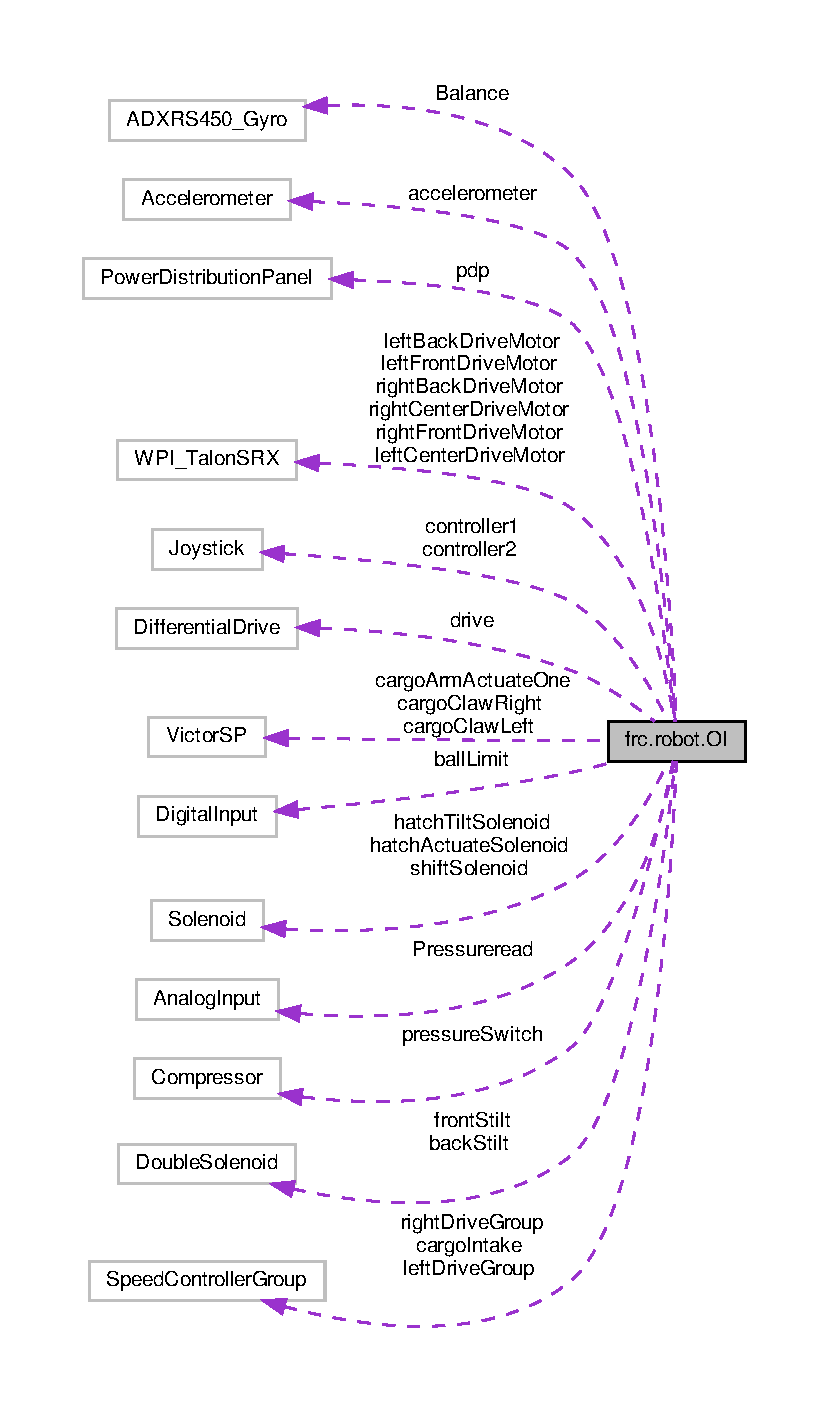
\includegraphics[height=550pt]{classfrc_1_1robot_1_1_o_i__coll__graph}
\end{center}
\end{figure}
\subsection*{Static Public Attributes}
\begin{DoxyCompactItemize}
\item 
\mbox{\Hypertarget{classfrc_1_1robot_1_1_o_i_a98d90326dfdaf14238d2f81c20c55f3f}\label{classfrc_1_1robot_1_1_o_i_a98d90326dfdaf14238d2f81c20c55f3f}} 
static Power\+Distribution\+Panel {\bfseries pdp} = new Power\+Distribution\+Panel(Robot\+Map.\+pdp\+C\+AN)
\item 
\mbox{\Hypertarget{classfrc_1_1robot_1_1_o_i_a06db411c1eebb80d10f685c57954bac9}\label{classfrc_1_1robot_1_1_o_i_a06db411c1eebb80d10f685c57954bac9}} 
static Joystick {\bfseries controller1} = new Joystick(Robot\+Map.\+controller\+One\+Port)
\item 
\mbox{\Hypertarget{classfrc_1_1robot_1_1_o_i_a749a3f830f90057dc4fd65e7f34a3251}\label{classfrc_1_1robot_1_1_o_i_a749a3f830f90057dc4fd65e7f34a3251}} 
static Joystick {\bfseries controller2} = new Joystick(Robot\+Map.\+controller\+Two\+Port)
\item 
\mbox{\Hypertarget{classfrc_1_1robot_1_1_o_i_a3f39e281419ebd60b94126e87e3ec81d}\label{classfrc_1_1robot_1_1_o_i_a3f39e281419ebd60b94126e87e3ec81d}} 
static W\+P\+I\+\_\+\+Talon\+S\+RX {\bfseries left\+Front\+Drive\+Motor} = new W\+P\+I\+\_\+\+Talon\+S\+RX(Robot\+Map.\+left\+Front\+Drive\+C\+AN)
\item 
\mbox{\Hypertarget{classfrc_1_1robot_1_1_o_i_a8c33a9f0b9e366e48abd23ab01907e18}\label{classfrc_1_1robot_1_1_o_i_a8c33a9f0b9e366e48abd23ab01907e18}} 
static W\+P\+I\+\_\+\+Talon\+S\+RX {\bfseries left\+Center\+Drive\+Motor} = new W\+P\+I\+\_\+\+Talon\+S\+RX(Robot\+Map.\+left\+Center\+Drive\+C\+AN)
\item 
\mbox{\Hypertarget{classfrc_1_1robot_1_1_o_i_a88080d092baf8ece2c22f2ceec4f6f8f}\label{classfrc_1_1robot_1_1_o_i_a88080d092baf8ece2c22f2ceec4f6f8f}} 
static W\+P\+I\+\_\+\+Talon\+S\+RX {\bfseries left\+Back\+Drive\+Motor} = new W\+P\+I\+\_\+\+Talon\+S\+RX(Robot\+Map.\+left\+Back\+Drive\+C\+AN)
\item 
\mbox{\Hypertarget{classfrc_1_1robot_1_1_o_i_ae055ab4ea5a306737c950b1bfddf7352}\label{classfrc_1_1robot_1_1_o_i_ae055ab4ea5a306737c950b1bfddf7352}} 
static W\+P\+I\+\_\+\+Talon\+S\+RX {\bfseries right\+Front\+Drive\+Motor} = new W\+P\+I\+\_\+\+Talon\+S\+RX(Robot\+Map.\+right\+Front\+Drive\+C\+AN)
\item 
\mbox{\Hypertarget{classfrc_1_1robot_1_1_o_i_a9be3279c18d1f3433d6b07c706eb1457}\label{classfrc_1_1robot_1_1_o_i_a9be3279c18d1f3433d6b07c706eb1457}} 
static W\+P\+I\+\_\+\+Talon\+S\+RX {\bfseries right\+Center\+Drive\+Motor} = new W\+P\+I\+\_\+\+Talon\+S\+RX(Robot\+Map.\+right\+Center\+Drive\+C\+AN)
\item 
\mbox{\Hypertarget{classfrc_1_1robot_1_1_o_i_a5f2937beffdc7dd1d937aaff36f20c1e}\label{classfrc_1_1robot_1_1_o_i_a5f2937beffdc7dd1d937aaff36f20c1e}} 
static W\+P\+I\+\_\+\+Talon\+S\+RX {\bfseries right\+Back\+Drive\+Motor} = new W\+P\+I\+\_\+\+Talon\+S\+RX(Robot\+Map.\+right\+Back\+Drive\+C\+AN)
\item 
\mbox{\Hypertarget{classfrc_1_1robot_1_1_o_i_a4f6b2dd823bad92cfaf2e9ecc7c0b1ca}\label{classfrc_1_1robot_1_1_o_i_a4f6b2dd823bad92cfaf2e9ecc7c0b1ca}} 
static Double\+Solenoid {\bfseries front\+Stilt} = new Double\+Solenoid(14, 2, 3)
\item 
\mbox{\Hypertarget{classfrc_1_1robot_1_1_o_i_a89667abb08d7721a47088f0218fd5afa}\label{classfrc_1_1robot_1_1_o_i_a89667abb08d7721a47088f0218fd5afa}} 
static Double\+Solenoid {\bfseries back\+Stilt} = new Double\+Solenoid(14, 6, 7)
\item 
\mbox{\Hypertarget{classfrc_1_1robot_1_1_o_i_a6d76241e542ab271366e4cb4bf7b5133}\label{classfrc_1_1robot_1_1_o_i_a6d76241e542ab271366e4cb4bf7b5133}} 
static Speed\+Controller\+Group {\bfseries left\+Drive\+Group} = new Speed\+Controller\+Group(left\+Center\+Drive\+Motor, left\+Back\+Drive\+Motor,left\+Front\+Drive\+Motor)
\item 
\mbox{\Hypertarget{classfrc_1_1robot_1_1_o_i_a1595c2b8ebd7e4e467027b2eb21983ee}\label{classfrc_1_1robot_1_1_o_i_a1595c2b8ebd7e4e467027b2eb21983ee}} 
static Speed\+Controller\+Group {\bfseries right\+Drive\+Group} = new Speed\+Controller\+Group(right\+Center\+Drive\+Motor, right\+Back\+Drive\+Motor)
\item 
\mbox{\Hypertarget{classfrc_1_1robot_1_1_o_i_a8527ec31aa37a3ff523e5ba857aba46f}\label{classfrc_1_1robot_1_1_o_i_a8527ec31aa37a3ff523e5ba857aba46f}} 
static Differential\+Drive {\bfseries drive} = new Differential\+Drive(left\+Drive\+Group, right\+Drive\+Group)
\item 
\mbox{\Hypertarget{classfrc_1_1robot_1_1_o_i_a63a56e8585378f6afe6f45facc98f494}\label{classfrc_1_1robot_1_1_o_i_a63a56e8585378f6afe6f45facc98f494}} 
static Solenoid {\bfseries shift\+Solenoid} = new Solenoid(Robot\+Map.\+P\+C\+M\+One\+C\+AN, Robot\+Map.\+shift\+Solenoid)
\item 
\mbox{\Hypertarget{classfrc_1_1robot_1_1_o_i_a232ad4f80d75cd3d48c2067251c59817}\label{classfrc_1_1robot_1_1_o_i_a232ad4f80d75cd3d48c2067251c59817}} 
static Solenoid {\bfseries hatch\+Actuate\+Solenoid} = new Solenoid(Robot\+Map.\+P\+C\+M\+One\+C\+AN, Robot\+Map.\+hatch\+Actuate)
\item 
\mbox{\Hypertarget{classfrc_1_1robot_1_1_o_i_aa8cdb6b236dfb9fead12621b4f42c274}\label{classfrc_1_1robot_1_1_o_i_aa8cdb6b236dfb9fead12621b4f42c274}} 
static Solenoid {\bfseries hatch\+Tilt\+Solenoid} = new Solenoid(Robot\+Map.\+P\+C\+M\+One\+C\+AN, Robot\+Map.\+hatch\+Tilt)
\item 
\mbox{\Hypertarget{classfrc_1_1robot_1_1_o_i_aeee9fe6efef4ea8f2558ccd2de43e71a}\label{classfrc_1_1robot_1_1_o_i_aeee9fe6efef4ea8f2558ccd2de43e71a}} 
static Victor\+SP {\bfseries cargo\+Arm\+Actuate\+One} = new Victor\+SP(Robot\+Map.\+cargo\+Arm\+Actuate\+One\+P\+WM)
\item 
\mbox{\Hypertarget{classfrc_1_1robot_1_1_o_i_a7ec725773fd1bb5dc4263980a232e75f}\label{classfrc_1_1robot_1_1_o_i_a7ec725773fd1bb5dc4263980a232e75f}} 
static Victor\+SP {\bfseries cargo\+Claw\+Left} = new Victor\+SP(Robot\+Map.\+cargo\+Claw\+Left\+Rotate\+P\+WM)
\item 
\mbox{\Hypertarget{classfrc_1_1robot_1_1_o_i_a32fd81c9a712924aa42a9eb74f278df1}\label{classfrc_1_1robot_1_1_o_i_a32fd81c9a712924aa42a9eb74f278df1}} 
static Victor\+SP {\bfseries cargo\+Claw\+Right} = new Victor\+SP(Robot\+Map.\+cargo\+Claw\+Right\+Rotate\+P\+WM)
\item 
\mbox{\Hypertarget{classfrc_1_1robot_1_1_o_i_a40d2adcc988805032885ba668fc6f86f}\label{classfrc_1_1robot_1_1_o_i_a40d2adcc988805032885ba668fc6f86f}} 
static Speed\+Controller\+Group {\bfseries cargo\+Intake} = new Speed\+Controller\+Group(cargo\+Claw\+Left, cargo\+Claw\+Right)
\item 
\mbox{\Hypertarget{classfrc_1_1robot_1_1_o_i_aebf7c01734a48f269b40f7b1f1125f10}\label{classfrc_1_1robot_1_1_o_i_aebf7c01734a48f269b40f7b1f1125f10}} 
static Digital\+Input {\bfseries ball\+Limit} = new Digital\+Input(Robot\+Map.\+ball\+Limit\+D\+IO)
\item 
\mbox{\Hypertarget{classfrc_1_1robot_1_1_o_i_a57e609e018f3013d5beb8bffa5771df0}\label{classfrc_1_1robot_1_1_o_i_a57e609e018f3013d5beb8bffa5771df0}} 
static Accelerometer {\bfseries accelerometer} = new Built\+In\+Accelerometer(Accelerometer.\+Range.\+k4G)
\item 
\mbox{\Hypertarget{classfrc_1_1robot_1_1_o_i_a68157a4a30cc0fae8bc36ae0ac999c82}\label{classfrc_1_1robot_1_1_o_i_a68157a4a30cc0fae8bc36ae0ac999c82}} 
static Compressor {\bfseries pressure\+Switch} = new Compressor()
\item 
\mbox{\Hypertarget{classfrc_1_1robot_1_1_o_i_a763d5acad9b29d4b29b0fff838059571}\label{classfrc_1_1robot_1_1_o_i_a763d5acad9b29d4b29b0fff838059571}} 
static Analog\+Input {\bfseries Pressureread} = new Analog\+Input(Robot\+Map.\+Pressure\+\_\+read)
\item 
\mbox{\Hypertarget{classfrc_1_1robot_1_1_o_i_a951d7ff102fca8319e5a9401a0f2214b}\label{classfrc_1_1robot_1_1_o_i_a951d7ff102fca8319e5a9401a0f2214b}} 
static A\+D\+X\+R\+S450\+\_\+\+Gyro {\bfseries Balance} = new A\+D\+X\+R\+S450\+\_\+\+Gyro()
\end{DoxyCompactItemize}


\subsection{Detailed Description}
This class is the glue that binds the controls on the physical operator interface to the commands and command groups that allow control of the robot. 

The documentation for this class was generated from the following file\+:\begin{DoxyCompactItemize}
\item 
src/main/java/frc/robot/O\+I.\+java\end{DoxyCompactItemize}

\hypertarget{classfrc_1_1robot_1_1_robot}{}\section{frc.\+robot.\+Robot Class Reference}
\label{classfrc_1_1robot_1_1_robot}\index{frc.\+robot.\+Robot@{frc.\+robot.\+Robot}}


Inheritance diagram for frc.\+robot.\+Robot\+:\nopagebreak
\begin{figure}[H]
\begin{center}
\leavevmode
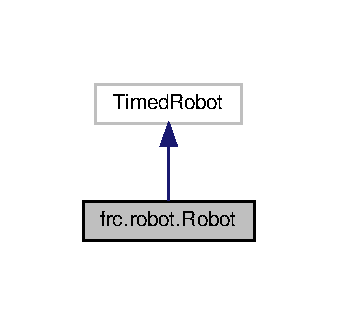
\includegraphics[width=162pt]{classfrc_1_1robot_1_1_robot__inherit__graph}
\end{center}
\end{figure}


Collaboration diagram for frc.\+robot.\+Robot\+:\nopagebreak
\begin{figure}[H]
\begin{center}
\leavevmode
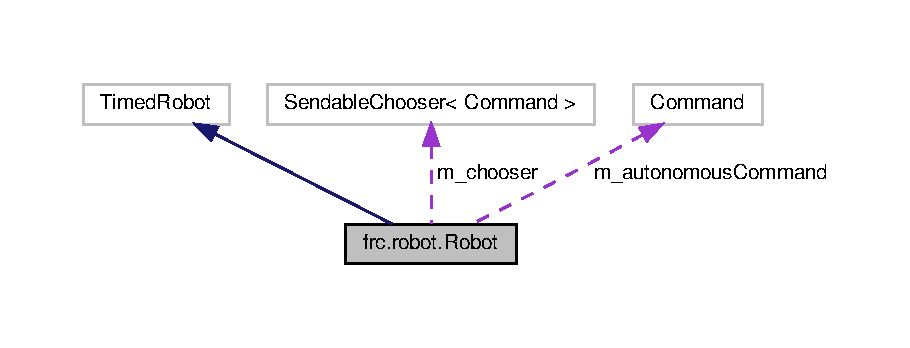
\includegraphics[width=350pt]{classfrc_1_1robot_1_1_robot__coll__graph}
\end{center}
\end{figure}
\subsection*{Public Member Functions}
\begin{DoxyCompactItemize}
\item 
\mbox{\Hypertarget{classfrc_1_1robot_1_1_robot_a1d28582cf3dc31568c3581f631c92f13}\label{classfrc_1_1robot_1_1_robot_a1d28582cf3dc31568c3581f631c92f13}} 
void {\bfseries robot\+Init} ()
\item 
\mbox{\Hypertarget{classfrc_1_1robot_1_1_robot_a7e63e32ebe8ad3d33bbc3b09092a9f1f}\label{classfrc_1_1robot_1_1_robot_a7e63e32ebe8ad3d33bbc3b09092a9f1f}} 
void {\bfseries robot\+Periodic} ()
\item 
\mbox{\Hypertarget{classfrc_1_1robot_1_1_robot_ac19810fbf26efd4cd47cbd7568b4ad2a}\label{classfrc_1_1robot_1_1_robot_ac19810fbf26efd4cd47cbd7568b4ad2a}} 
void {\bfseries disabled\+Init} ()
\item 
\mbox{\Hypertarget{classfrc_1_1robot_1_1_robot_a2bc1b0ce100e4783ba3d549e6ac07ae3}\label{classfrc_1_1robot_1_1_robot_a2bc1b0ce100e4783ba3d549e6ac07ae3}} 
void {\bfseries disabled\+Periodic} ()
\item 
\mbox{\Hypertarget{classfrc_1_1robot_1_1_robot_a5b1c022cd3e2b9f6e5dde62571839173}\label{classfrc_1_1robot_1_1_robot_a5b1c022cd3e2b9f6e5dde62571839173}} 
void {\bfseries autonomous\+Init} ()
\item 
void \hyperlink{classfrc_1_1robot_1_1_robot_a7dcfe7d0d65d1051eb095b8eb1aebd72}{autonomous\+Periodic} ()
\item 
\mbox{\Hypertarget{classfrc_1_1robot_1_1_robot_a209dbf07bfec75d73fa53126a8e31b88}\label{classfrc_1_1robot_1_1_robot_a209dbf07bfec75d73fa53126a8e31b88}} 
void {\bfseries teleop\+Init} ()
\item 
\mbox{\Hypertarget{classfrc_1_1robot_1_1_robot_ae807171661cbc29081bc10f06d6831e7}\label{classfrc_1_1robot_1_1_robot_ae807171661cbc29081bc10f06d6831e7}} 
void {\bfseries teleop\+Periodic} ()
\item 
\mbox{\Hypertarget{classfrc_1_1robot_1_1_robot_abd152f34b9f33d5cdf835aa61331f33e}\label{classfrc_1_1robot_1_1_robot_abd152f34b9f33d5cdf835aa61331f33e}} 
void {\bfseries test\+Periodic} ()
\end{DoxyCompactItemize}


\subsection{Member Function Documentation}
\mbox{\Hypertarget{classfrc_1_1robot_1_1_robot_a7dcfe7d0d65d1051eb095b8eb1aebd72}\label{classfrc_1_1robot_1_1_robot_a7dcfe7d0d65d1051eb095b8eb1aebd72}} 
\index{frc\+::robot\+::\+Robot@{frc\+::robot\+::\+Robot}!autonomous\+Periodic@{autonomous\+Periodic}}
\index{autonomous\+Periodic@{autonomous\+Periodic}!frc\+::robot\+::\+Robot@{frc\+::robot\+::\+Robot}}
\subsubsection{\texorpdfstring{autonomous\+Periodic()}{autonomousPeriodic()}}
{\footnotesize\ttfamily void frc.\+robot.\+Robot.\+autonomous\+Periodic (\begin{DoxyParamCaption}{ }\end{DoxyParamCaption})}

This function is called periodically during autonomous. 

The documentation for this class was generated from the following file\+:\begin{DoxyCompactItemize}
\item 
src/main/java/frc/robot/Robot.\+java\end{DoxyCompactItemize}

\hypertarget{classfrc_1_1robot_1_1_robot_map}{}\section{frc.\+robot.\+Robot\+Map Class Reference}
\label{classfrc_1_1robot_1_1_robot_map}\index{frc.\+robot.\+Robot\+Map@{frc.\+robot.\+Robot\+Map}}
\subsection*{Static Public Attributes}
\begin{DoxyCompactItemize}
\item 
\mbox{\Hypertarget{classfrc_1_1robot_1_1_robot_map_af7db1426412719318df15f9838b70198}\label{classfrc_1_1robot_1_1_robot_map_af7db1426412719318df15f9838b70198}} 
static int {\bfseries pdp\+C\+AN} = 6
\item 
\mbox{\Hypertarget{classfrc_1_1robot_1_1_robot_map_adf0118e5a9de03d6f71ea1e5a6a81cc9}\label{classfrc_1_1robot_1_1_robot_map_adf0118e5a9de03d6f71ea1e5a6a81cc9}} 
static int {\bfseries controller\+One\+Port} = 0
\item 
\mbox{\Hypertarget{classfrc_1_1robot_1_1_robot_map_a762ebcaa07378c37d88654506850e07f}\label{classfrc_1_1robot_1_1_robot_map_a762ebcaa07378c37d88654506850e07f}} 
static int {\bfseries controller\+Two\+Port} = 1
\item 
\mbox{\Hypertarget{classfrc_1_1robot_1_1_robot_map_a2e3dbfb148d6fa2b7f430614887217f0}\label{classfrc_1_1robot_1_1_robot_map_a2e3dbfb148d6fa2b7f430614887217f0}} 
static int {\bfseries left\+Front\+Drive\+C\+AN} = 15
\item 
\mbox{\Hypertarget{classfrc_1_1robot_1_1_robot_map_a9d04abf669a5ad42cb023e3ff3b56bcd}\label{classfrc_1_1robot_1_1_robot_map_a9d04abf669a5ad42cb023e3ff3b56bcd}} 
static int {\bfseries left\+Center\+Drive\+C\+AN} = 11
\item 
\mbox{\Hypertarget{classfrc_1_1robot_1_1_robot_map_a0f78f6850b0e060cc6acd88cc80ffa04}\label{classfrc_1_1robot_1_1_robot_map_a0f78f6850b0e060cc6acd88cc80ffa04}} 
static int {\bfseries left\+Back\+Drive\+C\+AN} = 12
\item 
\mbox{\Hypertarget{classfrc_1_1robot_1_1_robot_map_a4ca461a7ad91df180971974fd6abc236}\label{classfrc_1_1robot_1_1_robot_map_a4ca461a7ad91df180971974fd6abc236}} 
static int {\bfseries right\+Front\+Drive\+C\+AN} = 4
\item 
\mbox{\Hypertarget{classfrc_1_1robot_1_1_robot_map_a3ca36356410531e52126d2979ee17f13}\label{classfrc_1_1robot_1_1_robot_map_a3ca36356410531e52126d2979ee17f13}} 
static int {\bfseries right\+Center\+Drive\+C\+AN} = 13
\item 
\mbox{\Hypertarget{classfrc_1_1robot_1_1_robot_map_a0fb2fff6bf26e3f196d1cb02a89072c3}\label{classfrc_1_1robot_1_1_robot_map_a0fb2fff6bf26e3f196d1cb02a89072c3}} 
static int {\bfseries right\+Back\+Drive\+C\+AN} = 14
\item 
\mbox{\Hypertarget{classfrc_1_1robot_1_1_robot_map_aeb2d5ba2420aa4acb2c40f409580df82}\label{classfrc_1_1robot_1_1_robot_map_aeb2d5ba2420aa4acb2c40f409580df82}} 
static int {\bfseries shift\+Solenoid} = 0
\item 
\mbox{\Hypertarget{classfrc_1_1robot_1_1_robot_map_a7bec1963c7590911eb30697b0707d9b4}\label{classfrc_1_1robot_1_1_robot_map_a7bec1963c7590911eb30697b0707d9b4}} 
static int {\bfseries hatch\+Actuate} = 1
\item 
\mbox{\Hypertarget{classfrc_1_1robot_1_1_robot_map_a0c656cb43ea0fd37d6b94991e8473bf9}\label{classfrc_1_1robot_1_1_robot_map_a0c656cb43ea0fd37d6b94991e8473bf9}} 
static int {\bfseries hatch\+Tilt} = 2
\item 
\mbox{\Hypertarget{classfrc_1_1robot_1_1_robot_map_a207ae1f0df88fd16e01e6cb1b99f5208}\label{classfrc_1_1robot_1_1_robot_map_a207ae1f0df88fd16e01e6cb1b99f5208}} 
static int {\bfseries stilt\+Wheels\+Rotate\+Left\+C\+AN} = 6
\item 
\mbox{\Hypertarget{classfrc_1_1robot_1_1_robot_map_ab522f4712e7ed6ca72dc978e324fdc3e}\label{classfrc_1_1robot_1_1_robot_map_ab522f4712e7ed6ca72dc978e324fdc3e}} 
static int {\bfseries stilt\+Wheels\+Rotate\+Right\+C\+AN} = 8
\item 
\mbox{\Hypertarget{classfrc_1_1robot_1_1_robot_map_a49ce156a9e6ef017c0c6ebfead8998ad}\label{classfrc_1_1robot_1_1_robot_map_a49ce156a9e6ef017c0c6ebfead8998ad}} 
static int {\bfseries stilt\+Wheels\+Actuate\+Left\+C\+AN} = 7
\item 
\mbox{\Hypertarget{classfrc_1_1robot_1_1_robot_map_a8ff2304f39bd99c3b9705aa9977f21c2}\label{classfrc_1_1robot_1_1_robot_map_a8ff2304f39bd99c3b9705aa9977f21c2}} 
static int {\bfseries stilt\+Wheels\+Actuate\+Right\+C\+AN} = 9
\item 
\mbox{\Hypertarget{classfrc_1_1robot_1_1_robot_map_a42ebc770489a95382644455c79dfb3c6}\label{classfrc_1_1robot_1_1_robot_map_a42ebc770489a95382644455c79dfb3c6}} 
static int {\bfseries Cargo\+Claw\+Limit} = 0
\item 
\mbox{\Hypertarget{classfrc_1_1robot_1_1_robot_map_aaff9d0adef8e1f97db2ac47f985f044a}\label{classfrc_1_1robot_1_1_robot_map_aaff9d0adef8e1f97db2ac47f985f044a}} 
static int {\bfseries cargo\+Arm\+Actuate\+One\+P\+WM} = 9
\item 
\mbox{\Hypertarget{classfrc_1_1robot_1_1_robot_map_aa5824f279bf68bbd68ae1ea3087c4b67}\label{classfrc_1_1robot_1_1_robot_map_aa5824f279bf68bbd68ae1ea3087c4b67}} 
static int {\bfseries cargo\+Claw\+Left\+Rotate\+P\+WM} = 8
\item 
\mbox{\Hypertarget{classfrc_1_1robot_1_1_robot_map_a108c3b97c541e7ed5a152cea66981231}\label{classfrc_1_1robot_1_1_robot_map_a108c3b97c541e7ed5a152cea66981231}} 
static int {\bfseries cargo\+Claw\+Right\+Rotate\+P\+WM} = 0
\item 
\mbox{\Hypertarget{classfrc_1_1robot_1_1_robot_map_a79a848df56d706c787d9a4f9a0434e7f}\label{classfrc_1_1robot_1_1_robot_map_a79a848df56d706c787d9a4f9a0434e7f}} 
static int {\bfseries P\+C\+M\+One\+C\+AN} = 13
\item 
\mbox{\Hypertarget{classfrc_1_1robot_1_1_robot_map_a1667413e090171add7254ea3ada3a786}\label{classfrc_1_1robot_1_1_robot_map_a1667413e090171add7254ea3ada3a786}} 
static int {\bfseries P\+C\+M\+Two\+C\+AN} = 14
\item 
\mbox{\Hypertarget{classfrc_1_1robot_1_1_robot_map_a6b076d1f5509d27622dd6119d0cf87df}\label{classfrc_1_1robot_1_1_robot_map_a6b076d1f5509d27622dd6119d0cf87df}} 
static int {\bfseries back\+Stilt\+Extend\+One} = 0
\item 
\mbox{\Hypertarget{classfrc_1_1robot_1_1_robot_map_a8ca652cb3d064af4fa63e10d5f8a61ea}\label{classfrc_1_1robot_1_1_robot_map_a8ca652cb3d064af4fa63e10d5f8a61ea}} 
static int {\bfseries back\+Stilt\+Extend\+Two} = 1
\item 
\mbox{\Hypertarget{classfrc_1_1robot_1_1_robot_map_a8747738291bc40d22cac88f94783fc94}\label{classfrc_1_1robot_1_1_robot_map_a8747738291bc40d22cac88f94783fc94}} 
static int {\bfseries back\+Stilt\+Retract\+One} = 4
\item 
\mbox{\Hypertarget{classfrc_1_1robot_1_1_robot_map_a592884e36a4a4183b06712642911af62}\label{classfrc_1_1robot_1_1_robot_map_a592884e36a4a4183b06712642911af62}} 
static int {\bfseries back\+Stilt\+Retract\+Two} = 5
\item 
\mbox{\Hypertarget{classfrc_1_1robot_1_1_robot_map_ac82bec623ae333203544bc6e2b6affca}\label{classfrc_1_1robot_1_1_robot_map_ac82bec623ae333203544bc6e2b6affca}} 
static int {\bfseries front\+Stilt\+Extend\+One} = 2
\item 
\mbox{\Hypertarget{classfrc_1_1robot_1_1_robot_map_adaf591568f35bfea428a0daef88d2bd7}\label{classfrc_1_1robot_1_1_robot_map_adaf591568f35bfea428a0daef88d2bd7}} 
static int {\bfseries front\+Stilt\+Extend\+Two} = 3
\item 
\mbox{\Hypertarget{classfrc_1_1robot_1_1_robot_map_ac14d6b81afe55b4563fc122101e5d2a1}\label{classfrc_1_1robot_1_1_robot_map_ac14d6b81afe55b4563fc122101e5d2a1}} 
static int {\bfseries front\+Stilt\+Retract\+One} = 6
\item 
\mbox{\Hypertarget{classfrc_1_1robot_1_1_robot_map_a5c84f2be7047952afe472026a81a71db}\label{classfrc_1_1robot_1_1_robot_map_a5c84f2be7047952afe472026a81a71db}} 
static int {\bfseries front\+Stilt\+Retract\+Two} = 7
\item 
\mbox{\Hypertarget{classfrc_1_1robot_1_1_robot_map_a83f3eec03443af1dbe44492871796c92}\label{classfrc_1_1robot_1_1_robot_map_a83f3eec03443af1dbe44492871796c92}} 
static int {\bfseries ball\+Limit\+D\+IO} = 0
\item 
\mbox{\Hypertarget{classfrc_1_1robot_1_1_robot_map_a845df2a269757c4988d8a7b4721ae9a6}\label{classfrc_1_1robot_1_1_robot_map_a845df2a269757c4988d8a7b4721ae9a6}} 
static int {\bfseries pressure\+Switch} = 0
\item 
\mbox{\Hypertarget{classfrc_1_1robot_1_1_robot_map_a10cc39db919c29133e2bc774281804b0}\label{classfrc_1_1robot_1_1_robot_map_a10cc39db919c29133e2bc774281804b0}} 
static int {\bfseries Pressure\+\_\+read} = 0
\item 
\mbox{\Hypertarget{classfrc_1_1robot_1_1_robot_map_a628344048ec6bcb92c77be8e100d793a}\label{classfrc_1_1robot_1_1_robot_map_a628344048ec6bcb92c77be8e100d793a}} 
static int {\bfseries left\+Ramp\+One} = 0
\item 
\mbox{\Hypertarget{classfrc_1_1robot_1_1_robot_map_a8fe9ced14f786602722d0f571264364a}\label{classfrc_1_1robot_1_1_robot_map_a8fe9ced14f786602722d0f571264364a}} 
static int {\bfseries left\+Ramp\+Two} = 1
\item 
\mbox{\Hypertarget{classfrc_1_1robot_1_1_robot_map_a5858c523e9d55496c5879e1605dd8d09}\label{classfrc_1_1robot_1_1_robot_map_a5858c523e9d55496c5879e1605dd8d09}} 
static int {\bfseries right\+Ramp\+One} = 2
\item 
\mbox{\Hypertarget{classfrc_1_1robot_1_1_robot_map_a3b1dd0a30fea76ff6841bc16dca555ae}\label{classfrc_1_1robot_1_1_robot_map_a3b1dd0a30fea76ff6841bc16dca555ae}} 
static int {\bfseries right\+Ramp\+Two} = 3
\item 
\mbox{\Hypertarget{classfrc_1_1robot_1_1_robot_map_a563500240643659a777b4b64d648a57f}\label{classfrc_1_1robot_1_1_robot_map_a563500240643659a777b4b64d648a57f}} 
static int {\bfseries x\+Button} = 3
\item 
\mbox{\Hypertarget{classfrc_1_1robot_1_1_robot_map_a376cdfce24713ccddfd9ea4a9ae83772}\label{classfrc_1_1robot_1_1_robot_map_a376cdfce24713ccddfd9ea4a9ae83772}} 
static int {\bfseries y\+Button} = 4
\item 
\mbox{\Hypertarget{classfrc_1_1robot_1_1_robot_map_aed812a060e454b3406124a8a8ec95e15}\label{classfrc_1_1robot_1_1_robot_map_aed812a060e454b3406124a8a8ec95e15}} 
static int {\bfseries right\+StickX} = 4
\item 
\mbox{\Hypertarget{classfrc_1_1robot_1_1_robot_map_add774938fbf6b4cddcd06d376de27513}\label{classfrc_1_1robot_1_1_robot_map_add774938fbf6b4cddcd06d376de27513}} 
static int {\bfseries a\+Button} = 1
\item 
\mbox{\Hypertarget{classfrc_1_1robot_1_1_robot_map_abb2f8a028f422a7e8713d4be96075ce2}\label{classfrc_1_1robot_1_1_robot_map_abb2f8a028f422a7e8713d4be96075ce2}} 
static int {\bfseries b\+Button} = 2
\item 
\mbox{\Hypertarget{classfrc_1_1robot_1_1_robot_map_a712cd18ea686d732a170689f16882f47}\label{classfrc_1_1robot_1_1_robot_map_a712cd18ea686d732a170689f16882f47}} 
static int {\bfseries left\+Trigger} = 2
\item 
\mbox{\Hypertarget{classfrc_1_1robot_1_1_robot_map_acad41677decf390f9afe83b7d5d93e86}\label{classfrc_1_1robot_1_1_robot_map_acad41677decf390f9afe83b7d5d93e86}} 
static int {\bfseries left\+StickY} = 1
\item 
\mbox{\Hypertarget{classfrc_1_1robot_1_1_robot_map_a11fdb56e7e48fce0d79ce47500a8fb62}\label{classfrc_1_1robot_1_1_robot_map_a11fdb56e7e48fce0d79ce47500a8fb62}} 
static int {\bfseries right\+Trigger} = 3
\item 
\mbox{\Hypertarget{classfrc_1_1robot_1_1_robot_map_a5f7843ae11f89f4c181ff983d1124d20}\label{classfrc_1_1robot_1_1_robot_map_a5f7843ae11f89f4c181ff983d1124d20}} 
static int {\bfseries left\+Bumper} = 5
\item 
\mbox{\Hypertarget{classfrc_1_1robot_1_1_robot_map_ad604c407a262f8175b53bc4d4cc21438}\label{classfrc_1_1robot_1_1_robot_map_ad604c407a262f8175b53bc4d4cc21438}} 
static int {\bfseries right\+Bumper} = 6
\item 
\mbox{\Hypertarget{classfrc_1_1robot_1_1_robot_map_af4fcbac053dc99bf17bfad4073818f58}\label{classfrc_1_1robot_1_1_robot_map_af4fcbac053dc99bf17bfad4073818f58}} 
static int {\bfseries select\+Button} = 7
\item 
\mbox{\Hypertarget{classfrc_1_1robot_1_1_robot_map_ac74c72dbcfec76ff3773e99109ec8f1f}\label{classfrc_1_1robot_1_1_robot_map_ac74c72dbcfec76ff3773e99109ec8f1f}} 
static int {\bfseries start\+Button} = 8
\end{DoxyCompactItemize}


\subsection{Detailed Description}
The \hyperlink{classfrc_1_1robot_1_1_robot_map}{Robot\+Map} is a mapping from the ports sensors and actuators are wired into to a variable name. This provides flexibility changing wiring, makes checking the wiring easier and significantly reduces the number of magic numbers floating around. 

The documentation for this class was generated from the following file\+:\begin{DoxyCompactItemize}
\item 
src/main/java/frc/robot/Robot\+Map.\+java\end{DoxyCompactItemize}

\hypertarget{enumfrc_1_1robot_1_1_enums_1_1_shift}{}\section{frc.\+robot.\+Enums.\+Shift Enum Reference}
\label{enumfrc_1_1robot_1_1_enums_1_1_shift}\index{frc.\+robot.\+Enums.\+Shift@{frc.\+robot.\+Enums.\+Shift}}
\subsection*{Public Attributes}
\begin{DoxyCompactItemize}
\item 
\mbox{\Hypertarget{enumfrc_1_1robot_1_1_enums_1_1_shift_a66efd5ef2833112e313f06303c7c6003}\label{enumfrc_1_1robot_1_1_enums_1_1_shift_a66efd5ef2833112e313f06303c7c6003}} 
{\bfseries High\+\_\+\+Gear}
\item 
\mbox{\Hypertarget{enumfrc_1_1robot_1_1_enums_1_1_shift_a057c3458651c7a916da4241ae52b56d0}\label{enumfrc_1_1robot_1_1_enums_1_1_shift_a057c3458651c7a916da4241ae52b56d0}} 
{\bfseries Low\+\_\+\+Gear}
\end{DoxyCompactItemize}


The documentation for this enum was generated from the following file\+:\begin{DoxyCompactItemize}
\item 
src/main/java/frc/robot/\+Enums/Shift.\+java\end{DoxyCompactItemize}

\hypertarget{classfrc_1_1robot_1_1subsystems_1_1_stilts}{}\section{frc.\+robot.\+subsystems.\+Stilts Class Reference}
\label{classfrc_1_1robot_1_1subsystems_1_1_stilts}\index{frc.\+robot.\+subsystems.\+Stilts@{frc.\+robot.\+subsystems.\+Stilts}}
\subsection*{Static Public Member Functions}
\begin{DoxyCompactItemize}
\item 
static void \hyperlink{classfrc_1_1robot_1_1subsystems_1_1_stilts_af50dae1fe4775c73cefb856685f1e99a}{actuate\+Front} (\hyperlink{enumfrc_1_1robot_1_1_enums_1_1_lift___pistons}{Lift\+\_\+\+Pistons} \hyperlink{classfrc_1_1robot_1_1subsystems_1_1_stilts}{Stilts})
\item 
static void \hyperlink{classfrc_1_1robot_1_1subsystems_1_1_stilts_a450a870f59c6692eaac864def617ec71}{actuate\+Back} (\hyperlink{enumfrc_1_1robot_1_1_enums_1_1_lift___pistons}{Lift\+\_\+\+Pistons} \hyperlink{classfrc_1_1robot_1_1subsystems_1_1_stilts}{Stilts})
\end{DoxyCompactItemize}


\subsection{Detailed Description}
\begin{DoxyAuthor}{Author}
Nicholas Blackburn 
\end{DoxyAuthor}
\begin{DoxySeeAlso}{See also}
Switch statemints for both Sets of \hyperlink{classfrc_1_1robot_1_1subsystems_1_1_stilts}{Stilts} Lift\+\_\+\+Pistons is an Enum set is a list for case statements 
\end{DoxySeeAlso}


Definition at line 12 of file Stilts.\+java.



\subsection{Member Function Documentation}
\mbox{\Hypertarget{classfrc_1_1robot_1_1subsystems_1_1_stilts_a450a870f59c6692eaac864def617ec71}\label{classfrc_1_1robot_1_1subsystems_1_1_stilts_a450a870f59c6692eaac864def617ec71}} 
\index{frc\+::robot\+::subsystems\+::\+Stilts@{frc\+::robot\+::subsystems\+::\+Stilts}!actuate\+Back@{actuate\+Back}}
\index{actuate\+Back@{actuate\+Back}!frc\+::robot\+::subsystems\+::\+Stilts@{frc\+::robot\+::subsystems\+::\+Stilts}}
\subsubsection{\texorpdfstring{actuate\+Back()}{actuateBack()}}
{\footnotesize\ttfamily static void frc.\+robot.\+subsystems.\+Stilts.\+actuate\+Back (\begin{DoxyParamCaption}\item[{\hyperlink{enumfrc_1_1robot_1_1_enums_1_1_lift___pistons}{Lift\+\_\+\+Pistons}}]{Stilts }\end{DoxyParamCaption})\hspace{0.3cm}{\ttfamily [static]}}



Definition at line 28 of file Stilts.\+java.

\mbox{\Hypertarget{classfrc_1_1robot_1_1subsystems_1_1_stilts_af50dae1fe4775c73cefb856685f1e99a}\label{classfrc_1_1robot_1_1subsystems_1_1_stilts_af50dae1fe4775c73cefb856685f1e99a}} 
\index{frc\+::robot\+::subsystems\+::\+Stilts@{frc\+::robot\+::subsystems\+::\+Stilts}!actuate\+Front@{actuate\+Front}}
\index{actuate\+Front@{actuate\+Front}!frc\+::robot\+::subsystems\+::\+Stilts@{frc\+::robot\+::subsystems\+::\+Stilts}}
\subsubsection{\texorpdfstring{actuate\+Front()}{actuateFront()}}
{\footnotesize\ttfamily static void frc.\+robot.\+subsystems.\+Stilts.\+actuate\+Front (\begin{DoxyParamCaption}\item[{\hyperlink{enumfrc_1_1robot_1_1_enums_1_1_lift___pistons}{Lift\+\_\+\+Pistons}}]{Stilts }\end{DoxyParamCaption})\hspace{0.3cm}{\ttfamily [static]}}



Definition at line 14 of file Stilts.\+java.



The documentation for this class was generated from the following file\+:\begin{DoxyCompactItemize}
\item 
src/main/java/frc/robot/subsystems/\hyperlink{_stilts_8java}{Stilts.\+java}\end{DoxyCompactItemize}

\hypertarget{classfrc_1_1robot_1_1subsystems_1_1_teleop}{}\section{frc.\+robot.\+subsystems.\+Teleop Class Reference}
\label{classfrc_1_1robot_1_1subsystems_1_1_teleop}\index{frc.\+robot.\+subsystems.\+Teleop@{frc.\+robot.\+subsystems.\+Teleop}}
\subsection*{Static Public Member Functions}
\begin{DoxyCompactItemize}
\item 
static void \hyperlink{classfrc_1_1robot_1_1subsystems_1_1_teleop_ae90969b779b855da532e50706fa33401}{Periodic} ()
\end{DoxyCompactItemize}


\subsection{Detailed Description}


Definition at line 19 of file Teleop.\+java.



\subsection{Member Function Documentation}
\mbox{\Hypertarget{classfrc_1_1robot_1_1subsystems_1_1_teleop_ae90969b779b855da532e50706fa33401}\label{classfrc_1_1robot_1_1subsystems_1_1_teleop_ae90969b779b855da532e50706fa33401}} 
\index{frc\+::robot\+::subsystems\+::\+Teleop@{frc\+::robot\+::subsystems\+::\+Teleop}!Periodic@{Periodic}}
\index{Periodic@{Periodic}!frc\+::robot\+::subsystems\+::\+Teleop@{frc\+::robot\+::subsystems\+::\+Teleop}}
\subsubsection{\texorpdfstring{Periodic()}{Periodic()}}
{\footnotesize\ttfamily static void frc.\+robot.\+subsystems.\+Teleop.\+Periodic (\begin{DoxyParamCaption}{ }\end{DoxyParamCaption})\hspace{0.3cm}{\ttfamily [static]}}



Definition at line 21 of file Teleop.\+java.

Here is the call graph for this function\+:\nopagebreak
\begin{figure}[H]
\begin{center}
\leavevmode
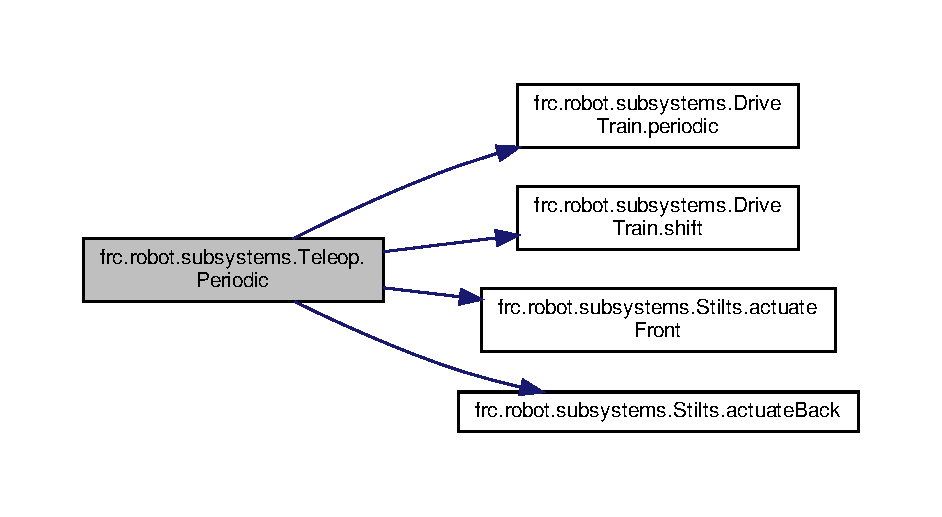
\includegraphics[width=350pt]{df/d7a/classfrc_1_1robot_1_1subsystems_1_1_teleop_ae90969b779b855da532e50706fa33401_cgraph}
\end{center}
\end{figure}


The documentation for this class was generated from the following file\+:\begin{DoxyCompactItemize}
\item 
src/main/java/frc/robot/subsystems/\hyperlink{_teleop_8java}{Teleop.\+java}\end{DoxyCompactItemize}

\hypertarget{classfrc_1_1robot_1_1subsystems_1_1_teleop___controller2}{}\section{frc.\+robot.\+subsystems.\+Teleop\+\_\+\+Controller2 Class Reference}
\label{classfrc_1_1robot_1_1subsystems_1_1_teleop___controller2}\index{frc.\+robot.\+subsystems.\+Teleop\+\_\+\+Controller2@{frc.\+robot.\+subsystems.\+Teleop\+\_\+\+Controller2}}
\subsection*{Static Public Member Functions}
\begin{DoxyCompactItemize}
\item 
\mbox{\Hypertarget{classfrc_1_1robot_1_1subsystems_1_1_teleop___controller2_a2943912b4181f00e084af67a56f6837f}\label{classfrc_1_1robot_1_1subsystems_1_1_teleop___controller2_a2943912b4181f00e084af67a56f6837f}} 
static void {\bfseries Teleop2} ()
\end{DoxyCompactItemize}


\subsection{Detailed Description}
\begin{DoxyAuthor}{Author}

\end{DoxyAuthor}
\begin{DoxySeeAlso}{See also}

\end{DoxySeeAlso}
\begin{DoxyVersion}{Version}
Button Maps Controller 2 (Operator controller) Left\+Bumper -\/ Sucks in ball Right\+Bumper -\/ Throws ball Left\+Trigger -\/ closes hatch Right\+Trigger -\/ opens hatch Left\+Stick -\/ moves \hyperlink{classfrc_1_1robot_1_1subsystems_1_1_cargo}{Cargo} arm Button X -\/ Stop \hyperlink{classfrc_1_1robot_1_1subsystems_1_1_cargo}{Cargo} arm 
\end{DoxyVersion}


The documentation for this class was generated from the following file\+:\begin{DoxyCompactItemize}
\item 
src/main/java/frc/robot/subsystems/Teleop\+\_\+\+Controller2.\+java\end{DoxyCompactItemize}

\chapter{File Documentation}
\hypertarget{_r_e_a_d_m_e_8md}{}\section{R\+E\+A\+D\+M\+E.\+md File Reference}
\label{_r_e_a_d_m_e_8md}\index{R\+E\+A\+D\+M\+E.\+md@{R\+E\+A\+D\+M\+E.\+md}}

\hypertarget{_hatch_8java}{}\section{src/main/java/frc/robot/\+Enums/\+Hatch.java File Reference}
\label{_hatch_8java}\index{src/main/java/frc/robot/\+Enums/\+Hatch.\+java@{src/main/java/frc/robot/\+Enums/\+Hatch.\+java}}
\subsection*{Classes}
\begin{DoxyCompactItemize}
\item 
enum \hyperlink{enumfrc_1_1robot_1_1_enums_1_1_hatch}{frc.\+robot.\+Enums.\+Hatch}
\end{DoxyCompactItemize}
\subsection*{Packages}
\begin{DoxyCompactItemize}
\item 
package \hyperlink{namespacefrc_1_1robot_1_1_enums}{frc.\+robot.\+Enums}
\end{DoxyCompactItemize}

\hypertarget{_lift___pistons_8java}{}\section{src/main/java/frc/robot/\+Enums/\+Lift\+\_\+\+Pistons.java File Reference}
\label{_lift___pistons_8java}\index{src/main/java/frc/robot/\+Enums/\+Lift\+\_\+\+Pistons.\+java@{src/main/java/frc/robot/\+Enums/\+Lift\+\_\+\+Pistons.\+java}}
\subsection*{Classes}
\begin{DoxyCompactItemize}
\item 
enum \hyperlink{enumfrc_1_1robot_1_1_enums_1_1_lift___pistons}{frc.\+robot.\+Enums.\+Lift\+\_\+\+Pistons}
\end{DoxyCompactItemize}
\subsection*{Packages}
\begin{DoxyCompactItemize}
\item 
package \hyperlink{namespacefrc_1_1robot_1_1_enums}{frc.\+robot.\+Enums}
\end{DoxyCompactItemize}

\hypertarget{_shift_8java}{}\section{src/main/java/frc/robot/\+Enums/\+Shift.java File Reference}
\label{_shift_8java}\index{src/main/java/frc/robot/\+Enums/\+Shift.\+java@{src/main/java/frc/robot/\+Enums/\+Shift.\+java}}
\subsection*{Classes}
\begin{DoxyCompactItemize}
\item 
enum \hyperlink{enumfrc_1_1robot_1_1_enums_1_1_shift}{frc.\+robot.\+Enums.\+Shift}
\end{DoxyCompactItemize}
\subsection*{Packages}
\begin{DoxyCompactItemize}
\item 
package \hyperlink{namespacefrc_1_1robot_1_1_enums}{frc.\+robot.\+Enums}
\end{DoxyCompactItemize}

\hypertarget{_main_8java}{}\section{src/main/java/frc/robot/\+Main.java File Reference}
\label{_main_8java}\index{src/main/java/frc/robot/\+Main.\+java@{src/main/java/frc/robot/\+Main.\+java}}
\subsection*{Classes}
\begin{DoxyCompactItemize}
\item 
class \hyperlink{classfrc_1_1robot_1_1_main}{frc.\+robot.\+Main}
\begin{DoxyCompactList}\small\item\em Do N\+OT add any static variables to this class, or any initialization at all. \end{DoxyCompactList}\end{DoxyCompactItemize}
\subsection*{Packages}
\begin{DoxyCompactItemize}
\item 
package \hyperlink{namespacefrc_1_1robot}{frc.\+robot}
\end{DoxyCompactItemize}

\hypertarget{_o_i_8java}{}\section{src/main/java/frc/robot/\+OI.java File Reference}
\label{_o_i_8java}\index{src/main/java/frc/robot/\+O\+I.\+java@{src/main/java/frc/robot/\+O\+I.\+java}}
\subsection*{Classes}
\begin{DoxyCompactItemize}
\item 
class \hyperlink{classfrc_1_1robot_1_1_o_i}{frc.\+robot.\+OI}
\begin{DoxyCompactList}\small\item\em This class is the glue that binds the controls on the physical operator interface to the commands and command groups that allow control of the robot. \end{DoxyCompactList}\end{DoxyCompactItemize}
\subsection*{Packages}
\begin{DoxyCompactItemize}
\item 
package \hyperlink{namespacefrc_1_1robot}{frc.\+robot}
\end{DoxyCompactItemize}

\hypertarget{_robot_8java}{}\section{src/main/java/frc/robot/\+Robot.java File Reference}
\label{_robot_8java}\index{src/main/java/frc/robot/\+Robot.\+java@{src/main/java/frc/robot/\+Robot.\+java}}
\subsection*{Classes}
\begin{DoxyCompactItemize}
\item 
class \hyperlink{classfrc_1_1robot_1_1_robot}{frc.\+robot.\+Robot}
\end{DoxyCompactItemize}
\subsection*{Packages}
\begin{DoxyCompactItemize}
\item 
package \hyperlink{namespacefrc_1_1robot}{frc.\+robot}
\end{DoxyCompactItemize}

\hypertarget{_robot_map_8java}{}\section{src/main/java/frc/robot/\+Robot\+Map.java File Reference}
\label{_robot_map_8java}\index{src/main/java/frc/robot/\+Robot\+Map.\+java@{src/main/java/frc/robot/\+Robot\+Map.\+java}}
\subsection*{Classes}
\begin{DoxyCompactItemize}
\item 
class \hyperlink{classfrc_1_1robot_1_1_robot_map}{frc.\+robot.\+Robot\+Map}
\begin{DoxyCompactList}\small\item\em The \hyperlink{classfrc_1_1robot_1_1_robot_map}{Robot\+Map} is a mapping from the ports sensors and actuators are wired into to a variable name. \end{DoxyCompactList}\end{DoxyCompactItemize}
\subsection*{Packages}
\begin{DoxyCompactItemize}
\item 
package \hyperlink{namespacefrc_1_1robot}{frc.\+robot}
\end{DoxyCompactItemize}

\hypertarget{_cargo_8java}{}\section{src/main/java/frc/robot/subsystems/\+Cargo.java File Reference}
\label{_cargo_8java}\index{src/main/java/frc/robot/subsystems/\+Cargo.\+java@{src/main/java/frc/robot/subsystems/\+Cargo.\+java}}
\subsection*{Classes}
\begin{DoxyCompactItemize}
\item 
class \hyperlink{classfrc_1_1robot_1_1subsystems_1_1_cargo}{frc.\+robot.\+subsystems.\+Cargo}
\end{DoxyCompactItemize}
\subsection*{Packages}
\begin{DoxyCompactItemize}
\item 
package \hyperlink{namespacefrc_1_1robot_1_1subsystems}{frc.\+robot.\+subsystems}
\end{DoxyCompactItemize}

\hypertarget{_drive_train_8java}{}\section{src/main/java/frc/robot/subsystems/\+Drive\+Train.java File Reference}
\label{_drive_train_8java}\index{src/main/java/frc/robot/subsystems/\+Drive\+Train.\+java@{src/main/java/frc/robot/subsystems/\+Drive\+Train.\+java}}
\subsection*{Classes}
\begin{DoxyCompactItemize}
\item 
class \hyperlink{classfrc_1_1robot_1_1subsystems_1_1_drive_train}{frc.\+robot.\+subsystems.\+Drive\+Train}
\end{DoxyCompactItemize}
\subsection*{Packages}
\begin{DoxyCompactItemize}
\item 
package \hyperlink{namespacefrc_1_1robot_1_1subsystems}{frc.\+robot.\+subsystems}
\end{DoxyCompactItemize}

\hypertarget{_hatch___control_8java}{}\section{src/main/java/frc/robot/subsystems/\+Hatch\+\_\+\+Control.java File Reference}
\label{_hatch___control_8java}\index{src/main/java/frc/robot/subsystems/\+Hatch\+\_\+\+Control.\+java@{src/main/java/frc/robot/subsystems/\+Hatch\+\_\+\+Control.\+java}}
\subsection*{Classes}
\begin{DoxyCompactItemize}
\item 
class \hyperlink{classfrc_1_1robot_1_1subsystems_1_1_hatch___control}{frc.\+robot.\+subsystems.\+Hatch\+\_\+\+Control}
\end{DoxyCompactItemize}
\subsection*{Packages}
\begin{DoxyCompactItemize}
\item 
package \hyperlink{namespacefrc_1_1robot_1_1subsystems}{frc.\+robot.\+subsystems}
\end{DoxyCompactItemize}

\hypertarget{_stilts_8java}{}\section{src/main/java/frc/robot/subsystems/\+Stilts.java File Reference}
\label{_stilts_8java}\index{src/main/java/frc/robot/subsystems/\+Stilts.\+java@{src/main/java/frc/robot/subsystems/\+Stilts.\+java}}
\subsection*{Classes}
\begin{DoxyCompactItemize}
\item 
class \hyperlink{classfrc_1_1robot_1_1subsystems_1_1_stilts}{frc.\+robot.\+subsystems.\+Stilts}
\end{DoxyCompactItemize}
\subsection*{Packages}
\begin{DoxyCompactItemize}
\item 
package \hyperlink{namespacefrc_1_1robot_1_1subsystems}{frc.\+robot.\+subsystems}
\end{DoxyCompactItemize}

\hypertarget{_teleop_8java}{}\section{src/main/java/frc/robot/subsystems/\+Teleop.java File Reference}
\label{_teleop_8java}\index{src/main/java/frc/robot/subsystems/\+Teleop.\+java@{src/main/java/frc/robot/subsystems/\+Teleop.\+java}}
\subsection*{Classes}
\begin{DoxyCompactItemize}
\item 
class \hyperlink{classfrc_1_1robot_1_1subsystems_1_1_teleop}{frc.\+robot.\+subsystems.\+Teleop}
\end{DoxyCompactItemize}
\subsection*{Packages}
\begin{DoxyCompactItemize}
\item 
package \hyperlink{namespacefrc_1_1robot_1_1subsystems}{frc.\+robot.\+subsystems}
\end{DoxyCompactItemize}

\hypertarget{_teleop___controller2_8java}{}\section{src/main/java/frc/robot/subsystems/\+Teleop\+\_\+\+Controller2.java File Reference}
\label{_teleop___controller2_8java}\index{src/main/java/frc/robot/subsystems/\+Teleop\+\_\+\+Controller2.\+java@{src/main/java/frc/robot/subsystems/\+Teleop\+\_\+\+Controller2.\+java}}
\subsection*{Classes}
\begin{DoxyCompactItemize}
\item 
class \hyperlink{classfrc_1_1robot_1_1subsystems_1_1_teleop___controller2}{frc.\+robot.\+subsystems.\+Teleop\+\_\+\+Controller2}
\end{DoxyCompactItemize}
\subsection*{Packages}
\begin{DoxyCompactItemize}
\item 
package \hyperlink{namespacefrc_1_1robot_1_1subsystems}{frc.\+robot.\+subsystems}
\end{DoxyCompactItemize}

%--- End generated contents ---

% Index
\backmatter
\newpage
\phantomsection
\clearemptydoublepage
\addcontentsline{toc}{chapter}{Index}
\printindex

\end{document}
